% ----------------------------------------------------------
% Calculadora de Execução Penal
% ----------------------------------------------------------
\chapter{CalPEC}
O presente Sistema Eletrônico para Cálculo do Processo de Execução Criminal foi desenvolvido com o objetivo de automatizar o cálculo de execução criminal, facilitar para os usuários o trâmite burocrático e garantir que tanto o apenado quanto o responsável pelo uso da ferramenta tenham resultados eficazes com o proposto, em que, com as informações necessárias, ele possa dar continuidade ao processo e usar como relatórios para fins de comprovação e avanços necessários.

A ideia foi garantir que os dados precisos de progressão de pena, remissões, detrações sejam calculados corretamente, de forma simples e intuitiva, que, além de entregar o que promete, ainda garante a experiência de usuário. A ferramenta de cálculo facilita o dia a dia do processo, a fim de minimizar os números de casos de ocorrências com falha durante o procedimento de cálculo criminal, causando riscos à segurança pública.

A calculadora surgiu a partir da observação das dificuldades enfrentadas por advogados e demais pessoas da área, especialmente em relação às falhas manuais durante o procedimento de cálculo sob a pena existente. Essas dificuldades são comuns entre o público da justiça e podem comprometer o desenvolvimento do processo burocrático de execução penal. Diante desse cenário, identificou-se a necessidade de desenvolver uma ferramenta que facilite o procedimento. Nesse contexto, a calculadora foi desenvolvida para atender a essa demanda, proporcionando: fluidez, eficácia no resultado dos cálculos submetidos.

\section{FUNCIONALIDADES PRINCIPAIS}
Diante das necessidades e dificuldades expostas, o presente sistema apresenta as seguintes soluções práticas: 

\begin{itemize}
    \item Registrar remição;
    \item Registrar detração;
    %\item Registrar unificação de pena;
    \item Exibir status de progressão;
    \item Calcular benefícios;
    \item Progressão de regime; 
    \item Cadastrar Condenado; e
    \item Cadastrar Advogado;
\end{itemize}

\section{MODELAGEM DO SISTEMA}

\subsection{Diagrama de casos de uso}
O Diagrama de Casos de Uso, apresentado na Figura~\ref{fig:casos-de-uso},
representa as interações entre o ator do sistema (o Advogado) e as funcionalidades disponíveis no CalPEC. O ator pode cadastrar-se, fazer login, cadastrar apenados, registrar execuções e remições, além de poder acompanhar o status de progressão. As relações de \textit{include} evidenciam que o cálculo de benefícios é acionado automaticamente pelo sistema sempre que uma execução é registrada ou uma remição é cadastrada, resultando na exibição do status de progressão de regime, atualizando-se a cada alteração sob a execução.

\begin{figure}[H]
    \caption{Diagrama de Casos de Uso.}
    \begin{center}
        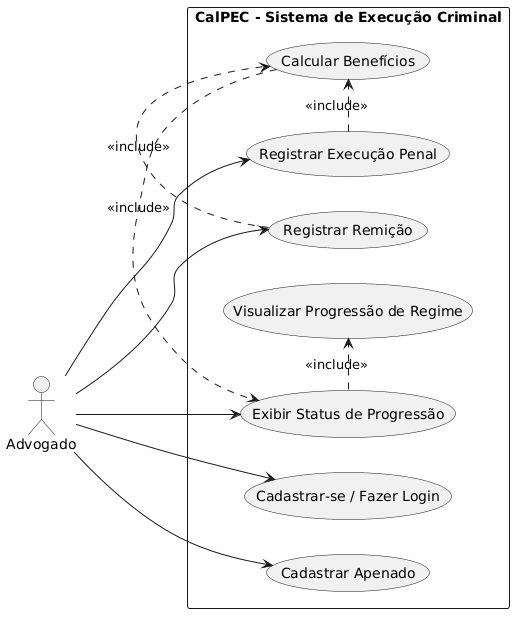
\includegraphics[width=0.6\textwidth]{imagens/diagramas/casos-de-uso.png}
    \end{center}
    \legend{Fonte: Elaborado pelo Autor}
    \label{fig:casos-de-uso}
\end{figure}

\newpage %COLOCADO PARA QUE O DIAGRAMA DE CLASSES FIQUE EM UMA PÁGINA SEPARADA, PARA MELHOR VISUALIZAÇÃO

\subsection{Diagrama de classes}
O Diagrama de Classes ilustrado na Figura~\ref{fig:classes}, representa a estrutura sistema, mostrando as quatro classes principais: \textit{Usuario}, \textit{Apenado}, \textit{Execucao} e \textit{Remicao}. Um usuário pode cadastrar múltiplos apenados e criar múltiplas execuções. Cada execução concentra os dados de tempo de pena, período de detração, regime inicial e os resultados do cálculo automático, como data de término, progressão de regime e data final de pena. A classe \textit{Remicao} registra as remições contínuas ao longo do cumprimento da pena, recalculando automaticamente a progressão a cada novo registro, conforme os benefícios realizados.

\begin{figure}[H]
    \caption{Diagrama de Classes.}
    \begin{center}
        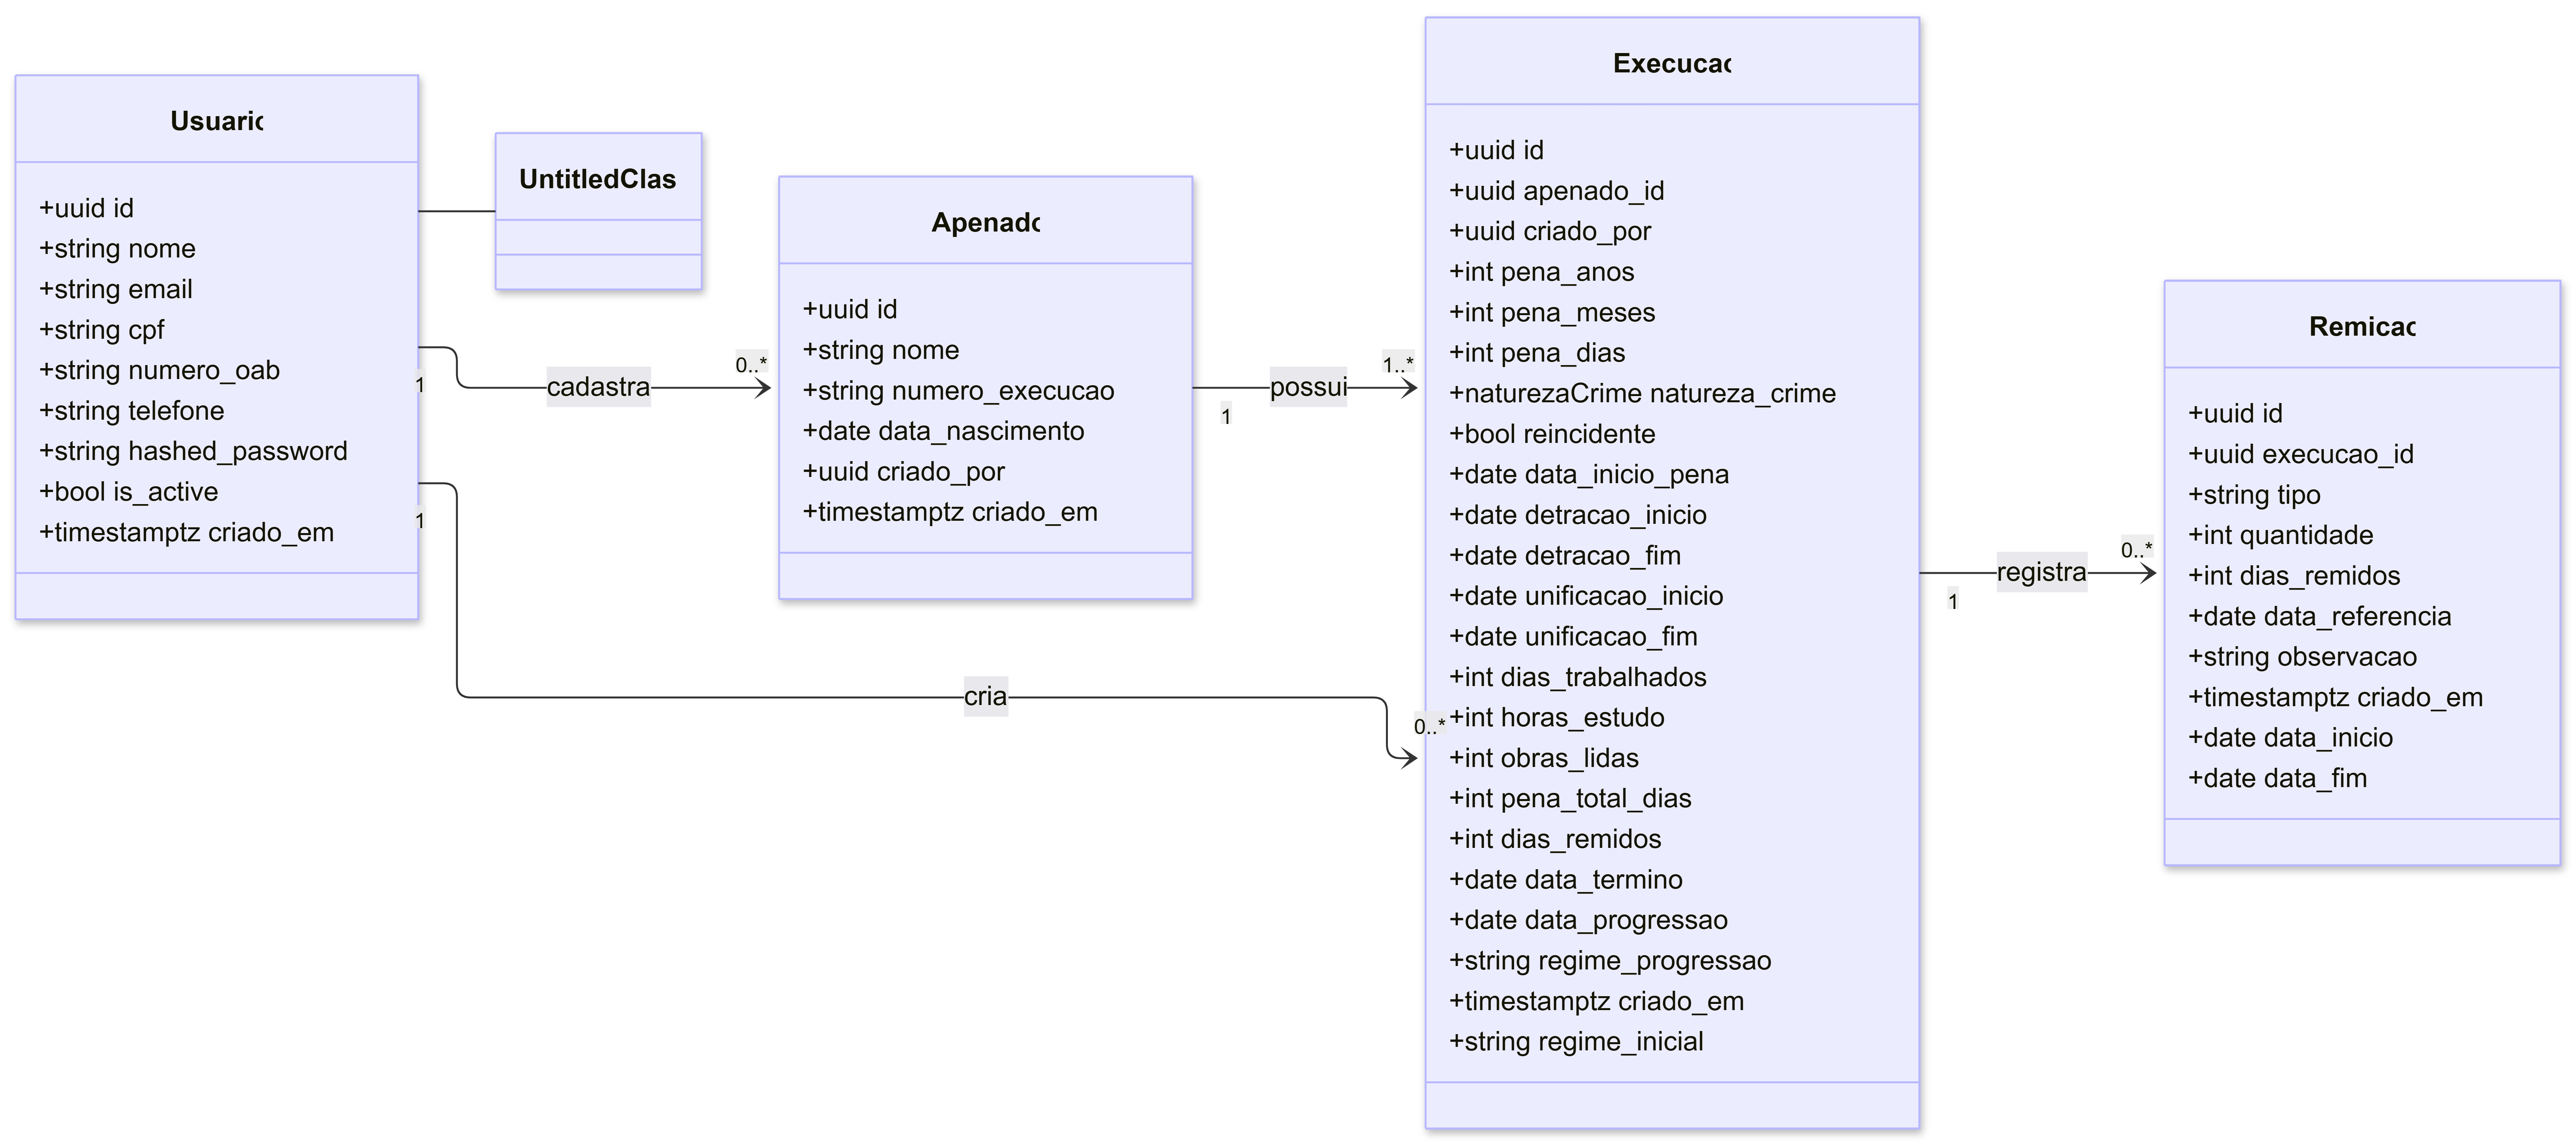
\includegraphics[width=1.1\textwidth]{imagens/diagramas/classes.png}
    \end{center}
    \legend{Fonte: Elaborado pelo Autor}
    \label{fig:classes}
\end{figure}

\newpage %COLOCADO PARA QUE O DIAGRAMA DE SEQUÊNCIA FIQUE EM UMA PÁGINA SEPARADA, PARA MELHOR VISUALIZAÇÃO
\subsection{Diagrama de sequência}
O Diagrama de Sequência demonstra o fluxo completo de interação entre o Advogado, o Sistema e o Banco de Dados, conforme mostra na Figura~\ref{fig:sequencia}. O fluxo inicia com o cadastro e login do usuário, seguido do cadastro do apenado e do registro da execução penal, momento em que o sistema realiza automaticamente o cálculo da pena total, detração, remição inicial e progressão de regime, persistindo o
resultado no banco de dados. Por fim, o diagrama ilustra o registro de novas remições ao longo do tempo, que realizam o recálculo automático da progressão e do término da pena.

\begin{figure}[H]
    \caption{Diagrama de Sequência.}
    \begin{center}
        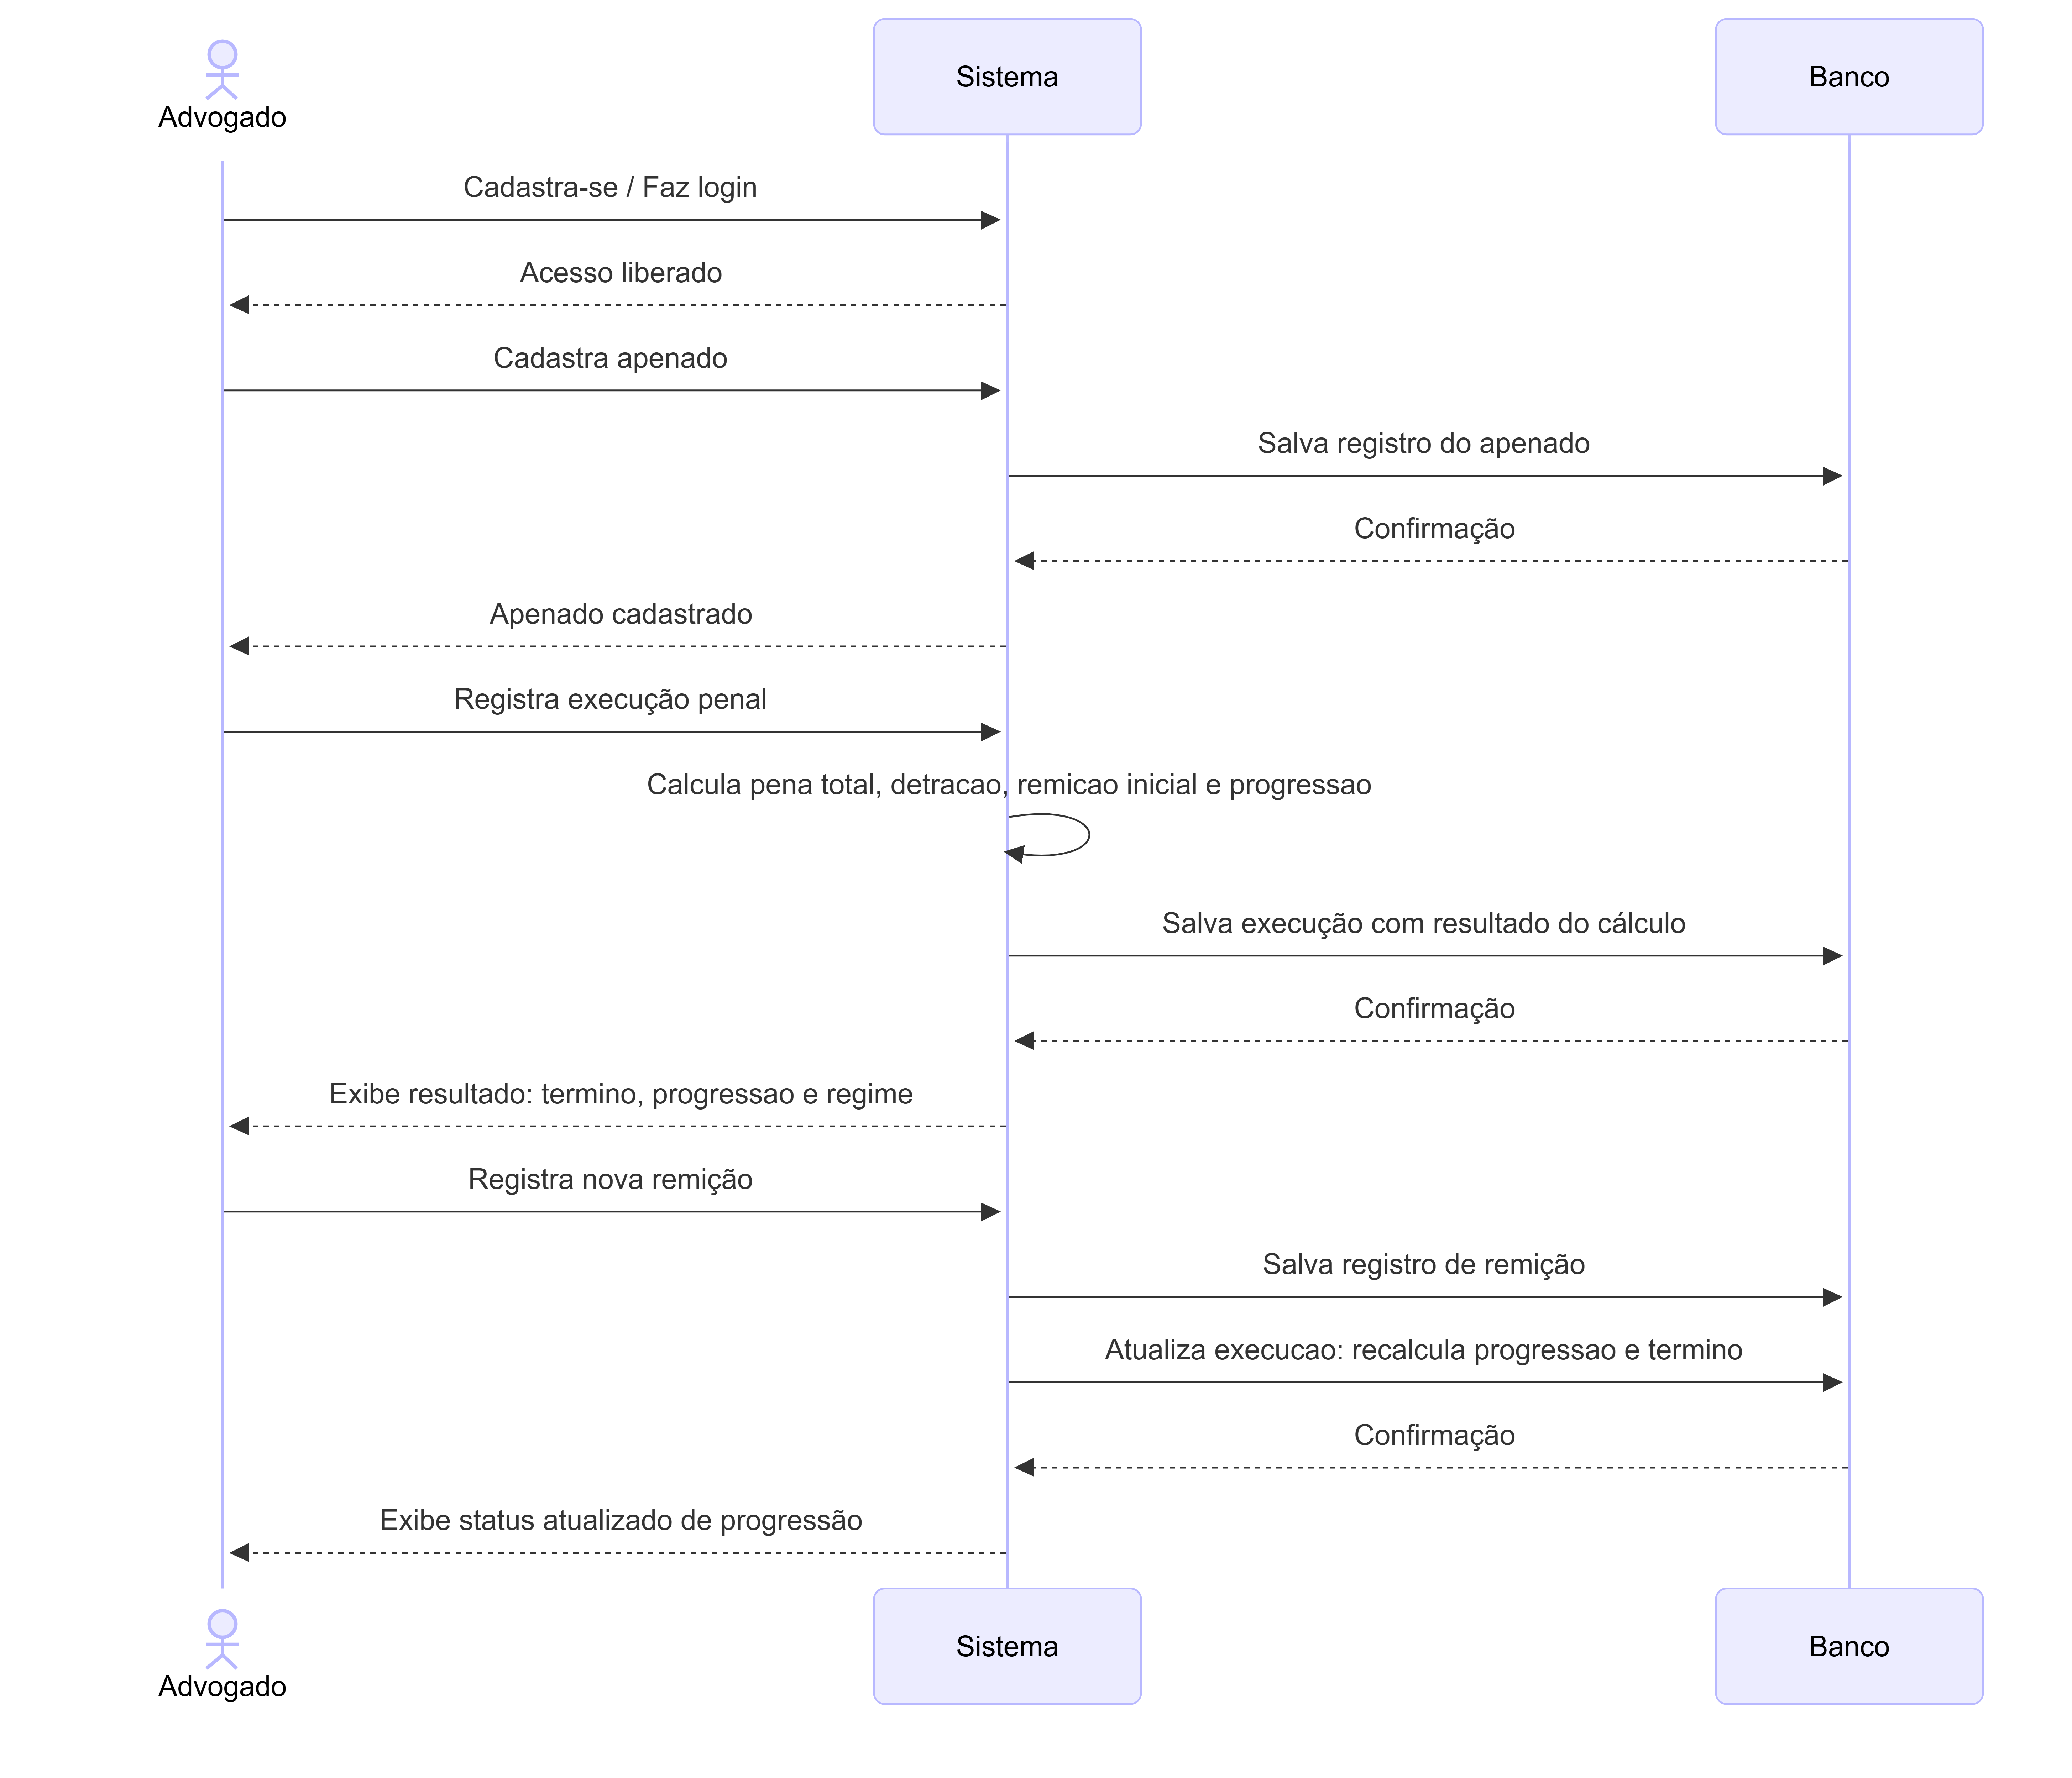
\includegraphics[width=1.0\textwidth]{imagens/diagramas/sequencia.png}
    \end{center}
    \legend{Fonte: Elaborado pelo Autor}
    \label{fig:sequencia}
\end{figure}

\newpage %COLOCADO PARA QUE O DIAGRAMA DER FIQUE EM UMA PÁGINA SEPARADA, PARA MELHOR VISUALIZAÇÃO
\subsection{Diagrama de entidade-relacionamento}
O Diagrama Entidade-Relacionamento, descreve a estrutura do banco de dados do sistema CalPEC. A entidade central é \textit{EXECUCAO}, que se relaciona diretamente com \textit{APENADO}, \textit{USUARIO} e \textit{REMICAO}, Figura~\ref{fig:der}. A entidade \textit{USUARIO} representa o advogado cadastrado no sistema, responsável pelo cadastro dos apenados e pela criação das execuções. A entidade \textit{REMICAO} registra individualmente cada atividade de remição realizada pelo apenado, mantendo o histórico completo para fins de cálculo e comprovação.

\begin{figure}[H]
    \caption{Diagrama Entidade-Relacionamento.}
    \begin{center}
        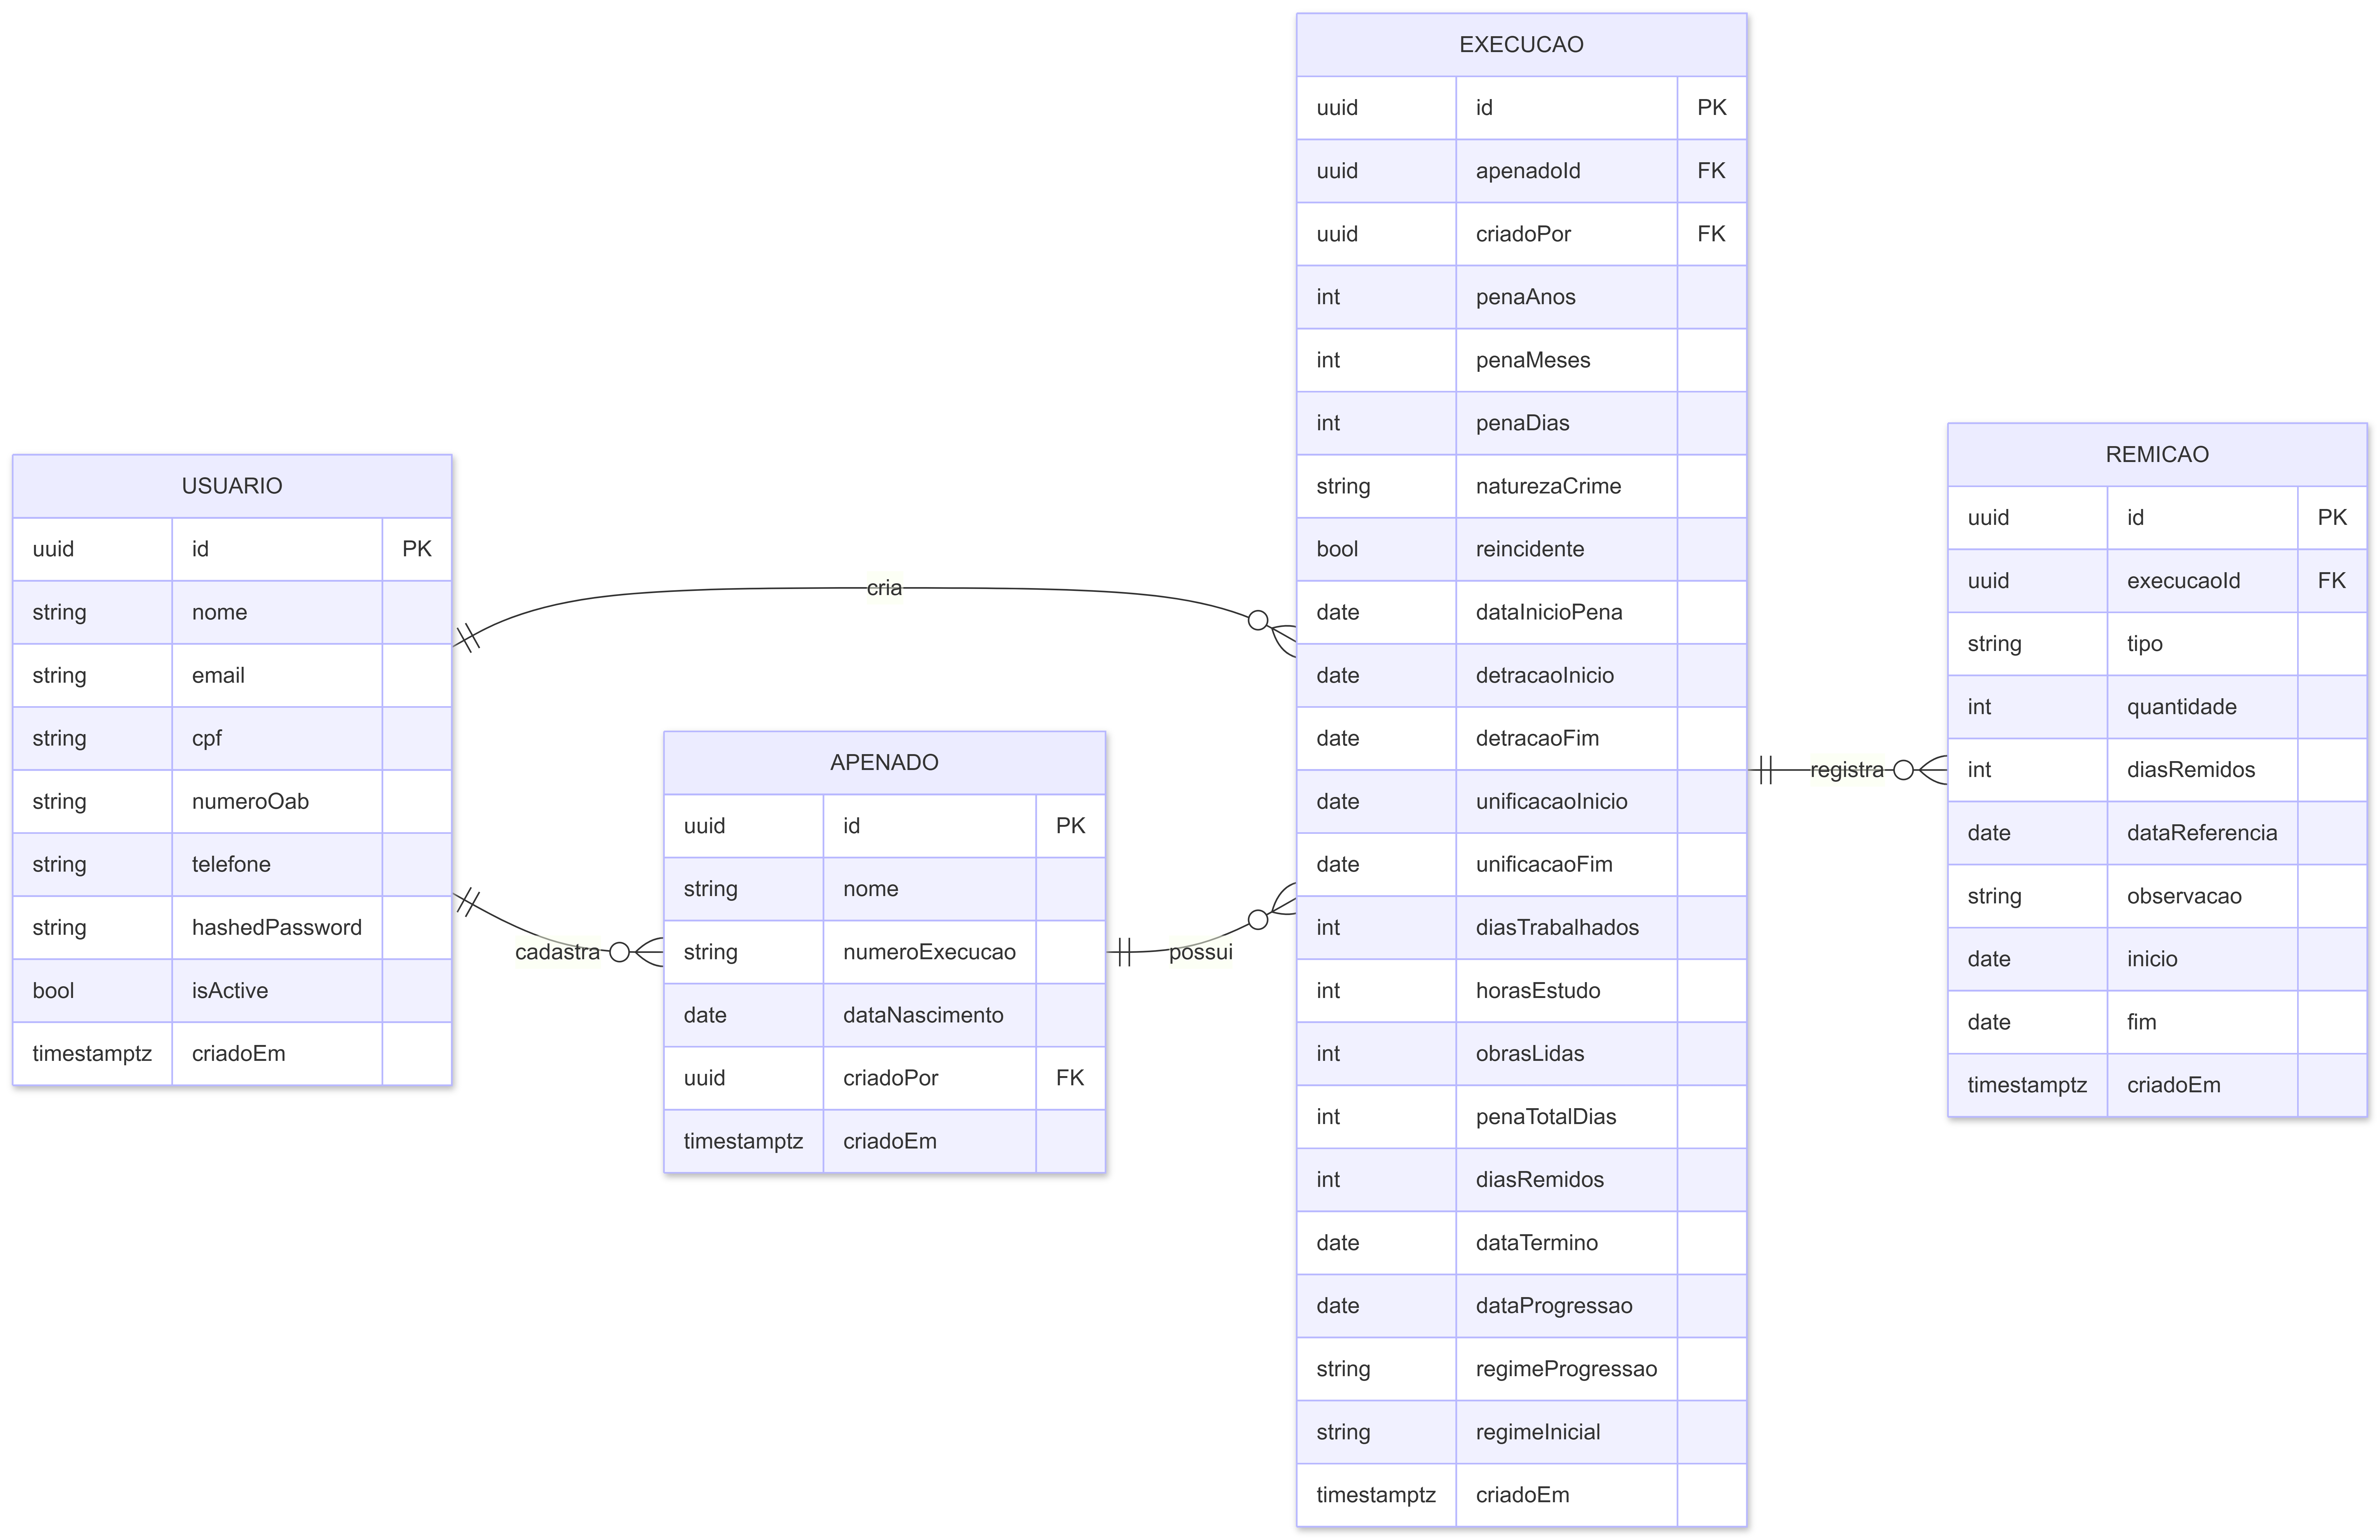
\includegraphics[width=1.0\textwidth]{imagens/diagramas/der.png}
    \end{center}
    \legend{Fonte: Elaborado pelo Autor}
    \label{fig:der}
\end{figure}

\newpage %SEÇÃO DE TELAS DO SISTEMA

\section{TELAS DO SISTEMA}
\subsection{Tela de login}
A Figura~\ref{fig:login} exibe a tela de login da calculadora, na qual o usuário pode realizar o login, caso já seja cadastrado, ou pode cadastrar-se clicando abaixo de "Cadastre-se". A tela de login é o ponto de partida para acessar o sistema. Depois de realizar o cadastro, preenchendo o formulário com os dados solicitados(nome completo, email, CPF, n°OAB, telefone e senha de acesso), o usuário é redirecionado para a tela de login para acessar o sistema. O login é realizado por meio do e-mail/CPF e senha cadastrados.
\begin{figure}[H]
    \caption{Tela de Login.}
    \begin{center}
        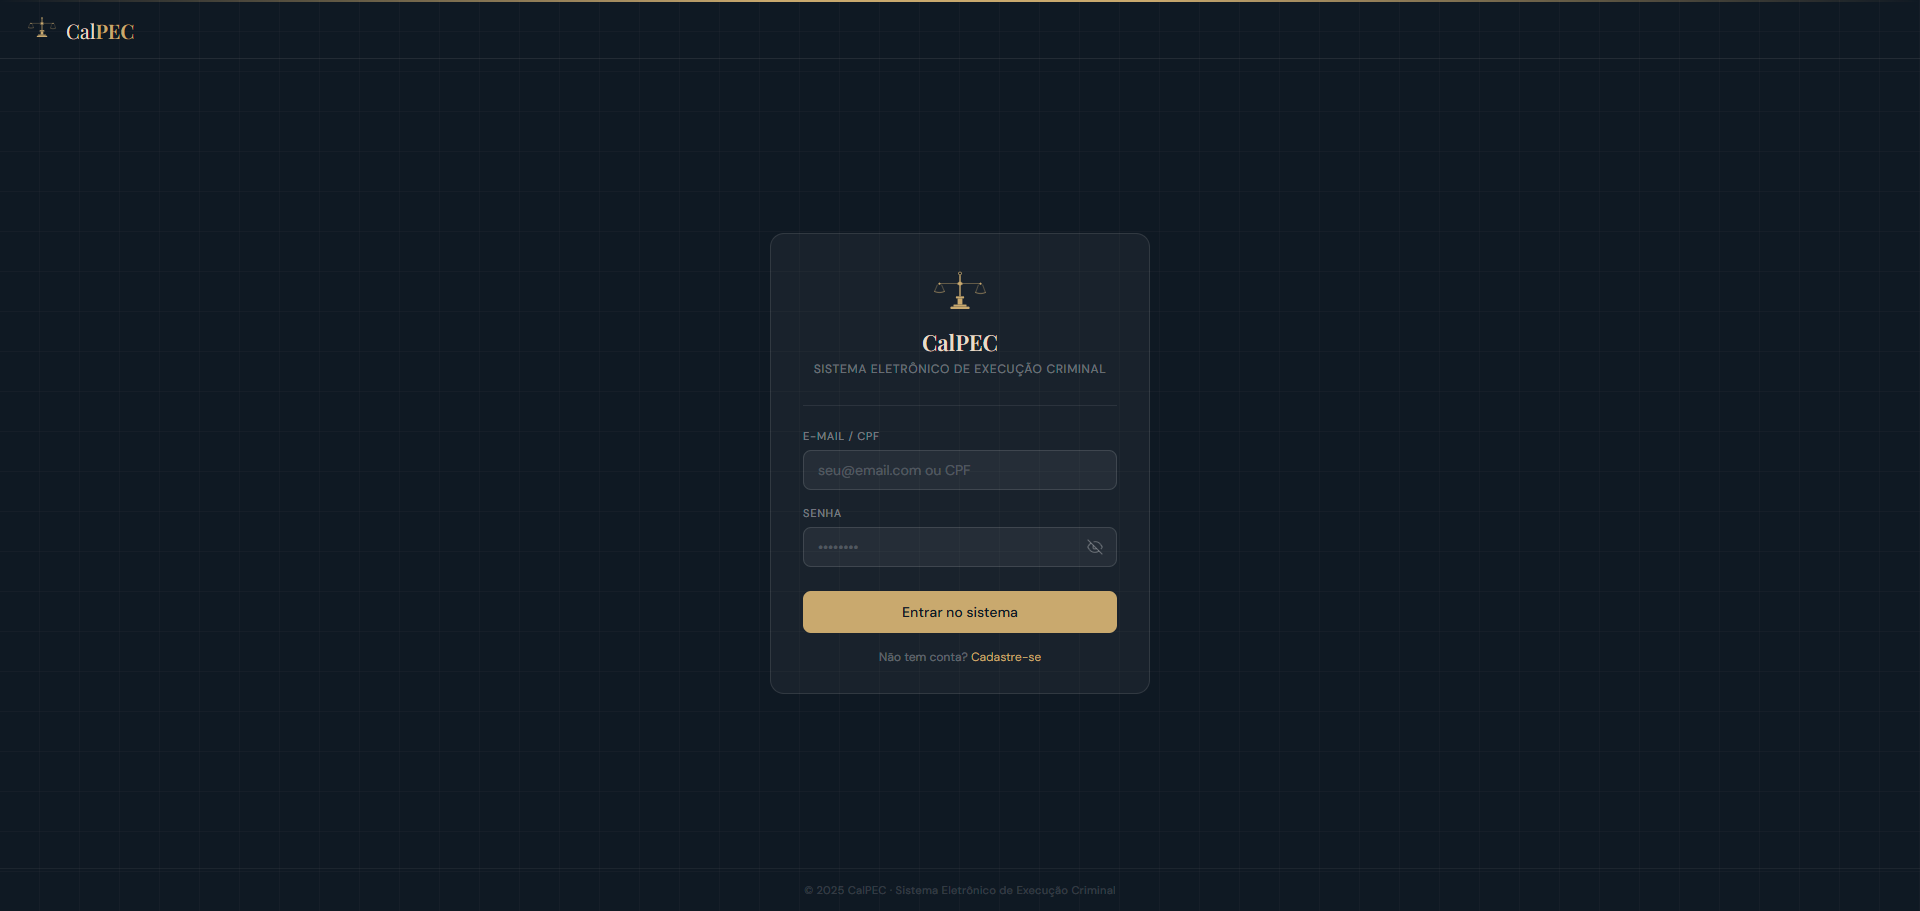
\includegraphics[width=1.0\textwidth]{imagens/prototipo/login.png}
    \end{center}
    \legend{Fonte: Elaborado pelo Autor}
    \label{fig:login}
\end{figure}

\subsection{Cadastro de usuário}
A Figura~\ref{fig:cadastro-usuario} apresenta a tela de cadastro do advogado no sistema. Por ser o único perfil de usuário do CalPEC, o cadastro é realizado diretamente nessa tela, que solicita as informações necessárias para identificação e acesso: nome completo, e-mail, CPF, número da OAB, telefone e senha. Após o cadastro, o advogado é redirecionado para a tela de login para acessar o sistema.

\begin{figure}[H]
    \caption{Cadastro de Usuário.}
    \begin{center}
        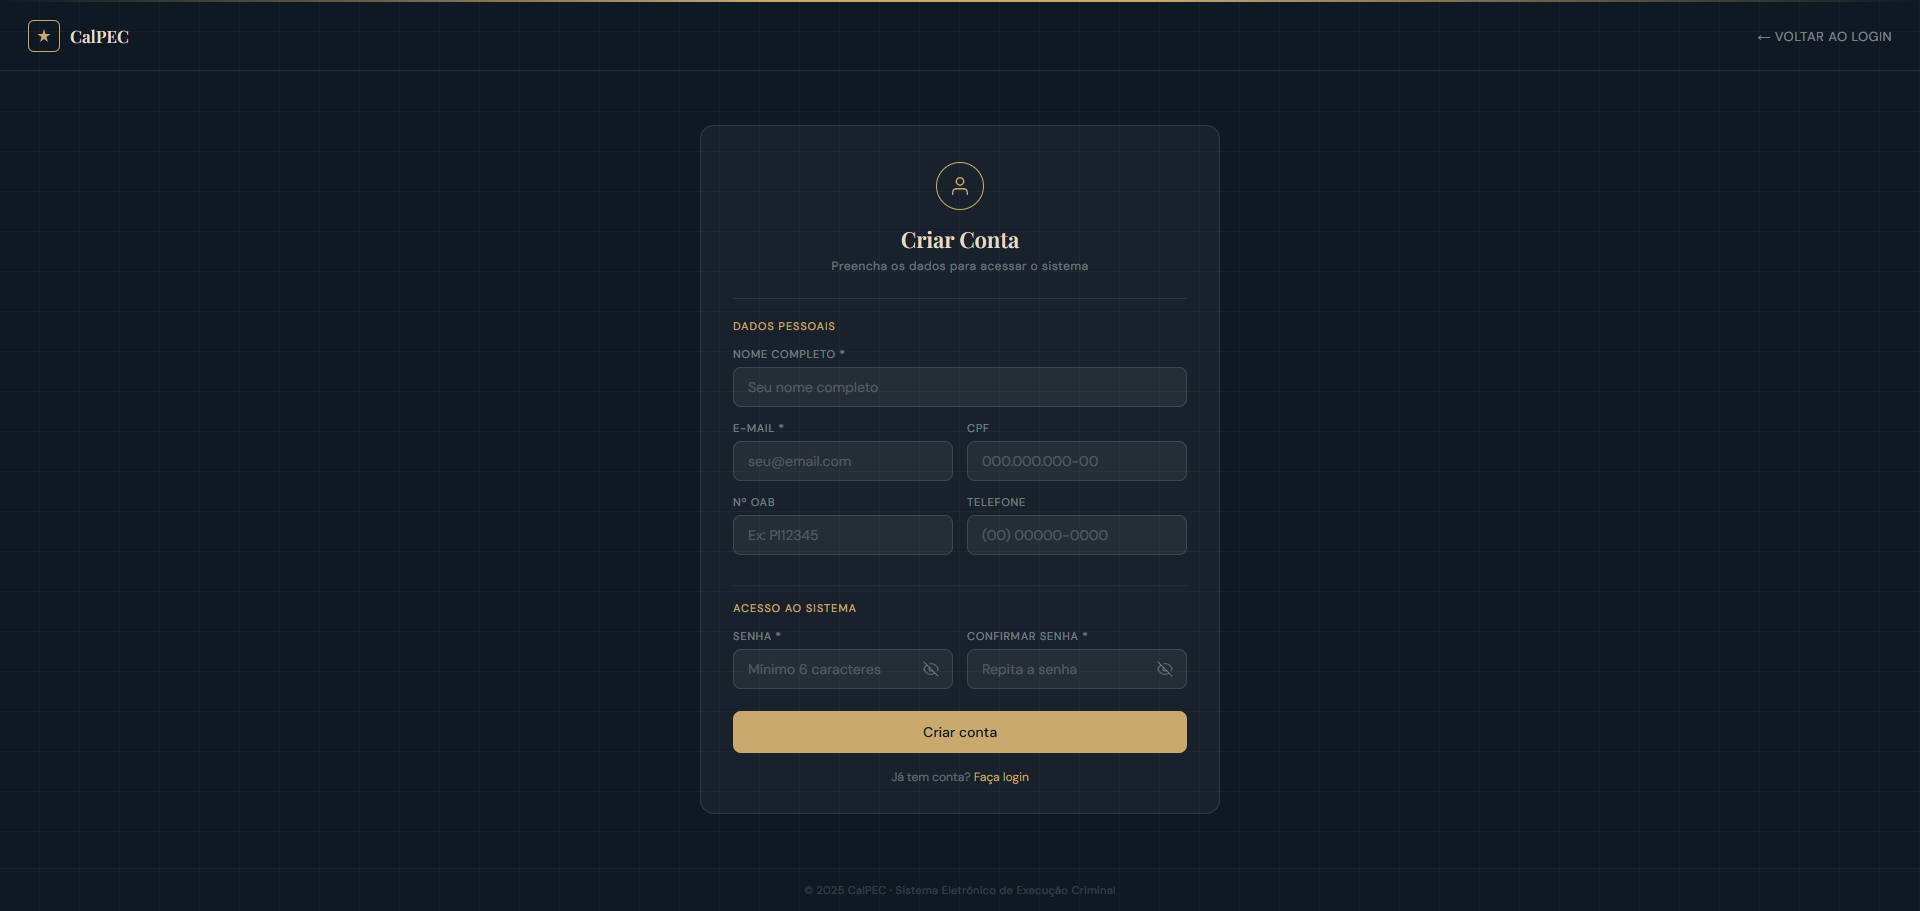
\includegraphics[width=1.0\textwidth]{imagens/prototipo/cadastrar-usuario.png}
    \end{center}
    \legend{Fonte: Elaborado pelo Autor}
    \label{fig:cadastro-usuario}
\end{figure}

\subsection{Tela inicial}
Após efetuar o login, o usuário navega até a página inicial do sistema, conforme a Figura~\ref{fig:tela-inicial}. A Tela Inicial apresenta, com clareza, as áreas de Apenados e Execuções do sistema, enfatizando o objetivo principal do sistema. Ao clicar em uma das opções, o sistema carrega um pop-up de listagem, onde o usuário pode navegar para o registro de uma execução ou para o registro de um condenado.

\begin{figure}[H]
    \caption{Tela Inicial.}
    \begin{center}
        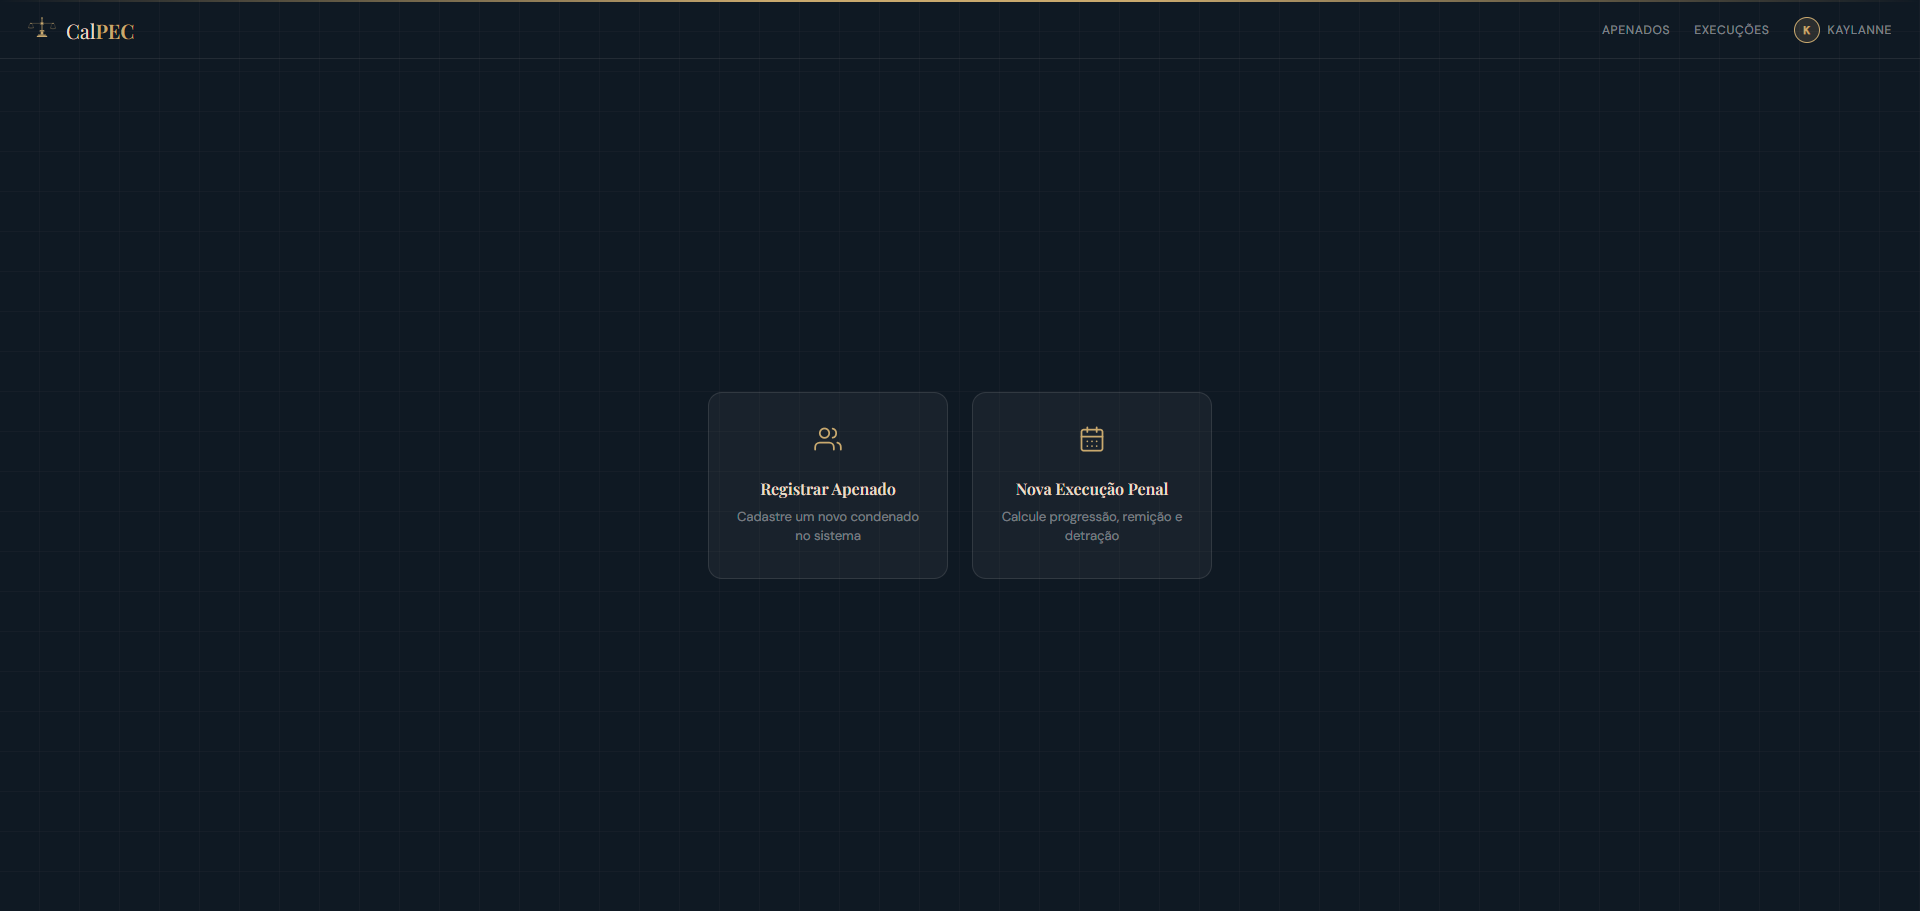
\includegraphics[width=1.0\textwidth]{imagens/prototipo/tela-inicial.png}
    \end{center}
    \legend{Fonte: Elaborado pelo Autor}
    \label{fig:tela-inicial}
\end{figure}

\subsection{Listar apenados}
A Figura~\ref{fig:list-apenados} exibe a tela de listagem dos apenados cadastrados no sistema. Nela, o advogado tem uma visão geral de todos os apenados registrados, podendo acessar os detalhes de cada um, editar suas informações ou navegar para o registro de uma nova execução penal vinculada ao apenado selecionado.

\begin{figure}[H]
    \caption{Listar Apenados.}
    \begin{center}
        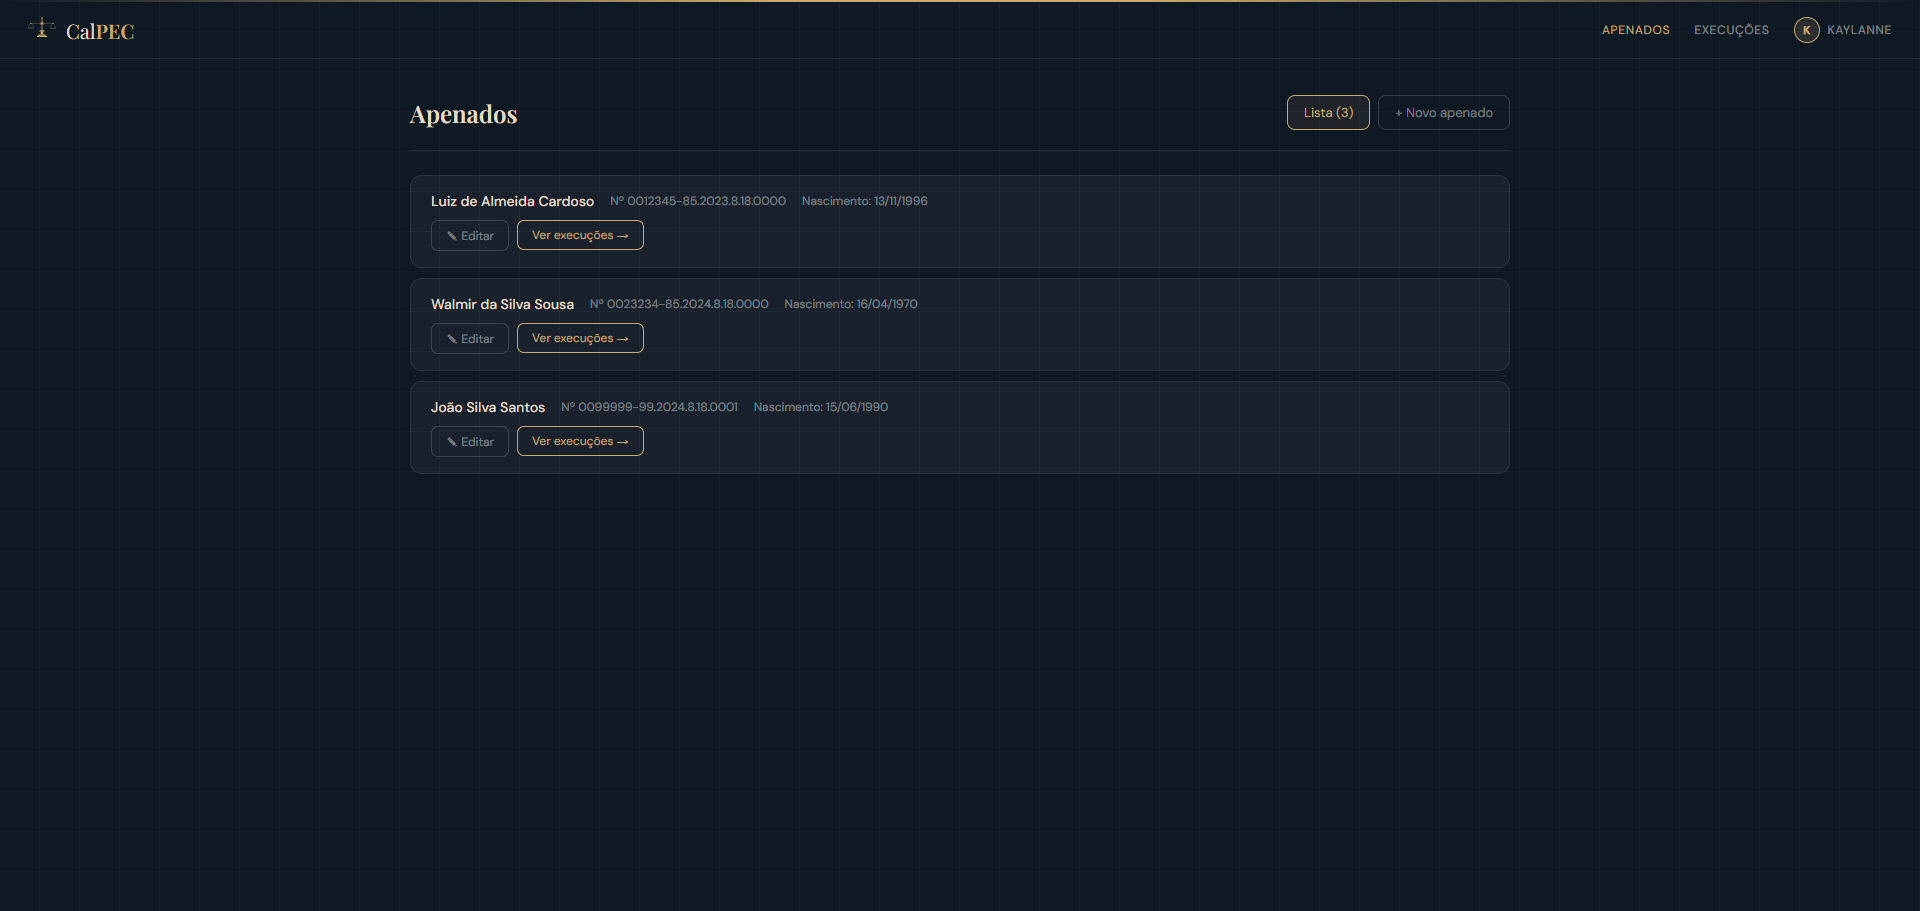
\includegraphics[width=1.0\textwidth]{imagens/prototipo/list-apenados.png}
    \end{center}
    \legend{Fonte: Elaborado pelo Autor}
    \label{fig:list-apenados}
\end{figure}

\subsection{Registrar apenado}
Ao clicar em "registrar apenado", o sistema navega até a página de cadastro do condenado, conforme a Figura~\ref{fig:tela-apenado}. Os campos necessários para preenchimento são: nome completo, número da execução ou processo e a data de nascimento do condenado. A idade de um apenado é um fator importante para a análise de benefícios específicos e condições de cumprimento da pena.

\begin{figure}[H]
    \caption{Registrar Apenado.}
    \begin{center}
        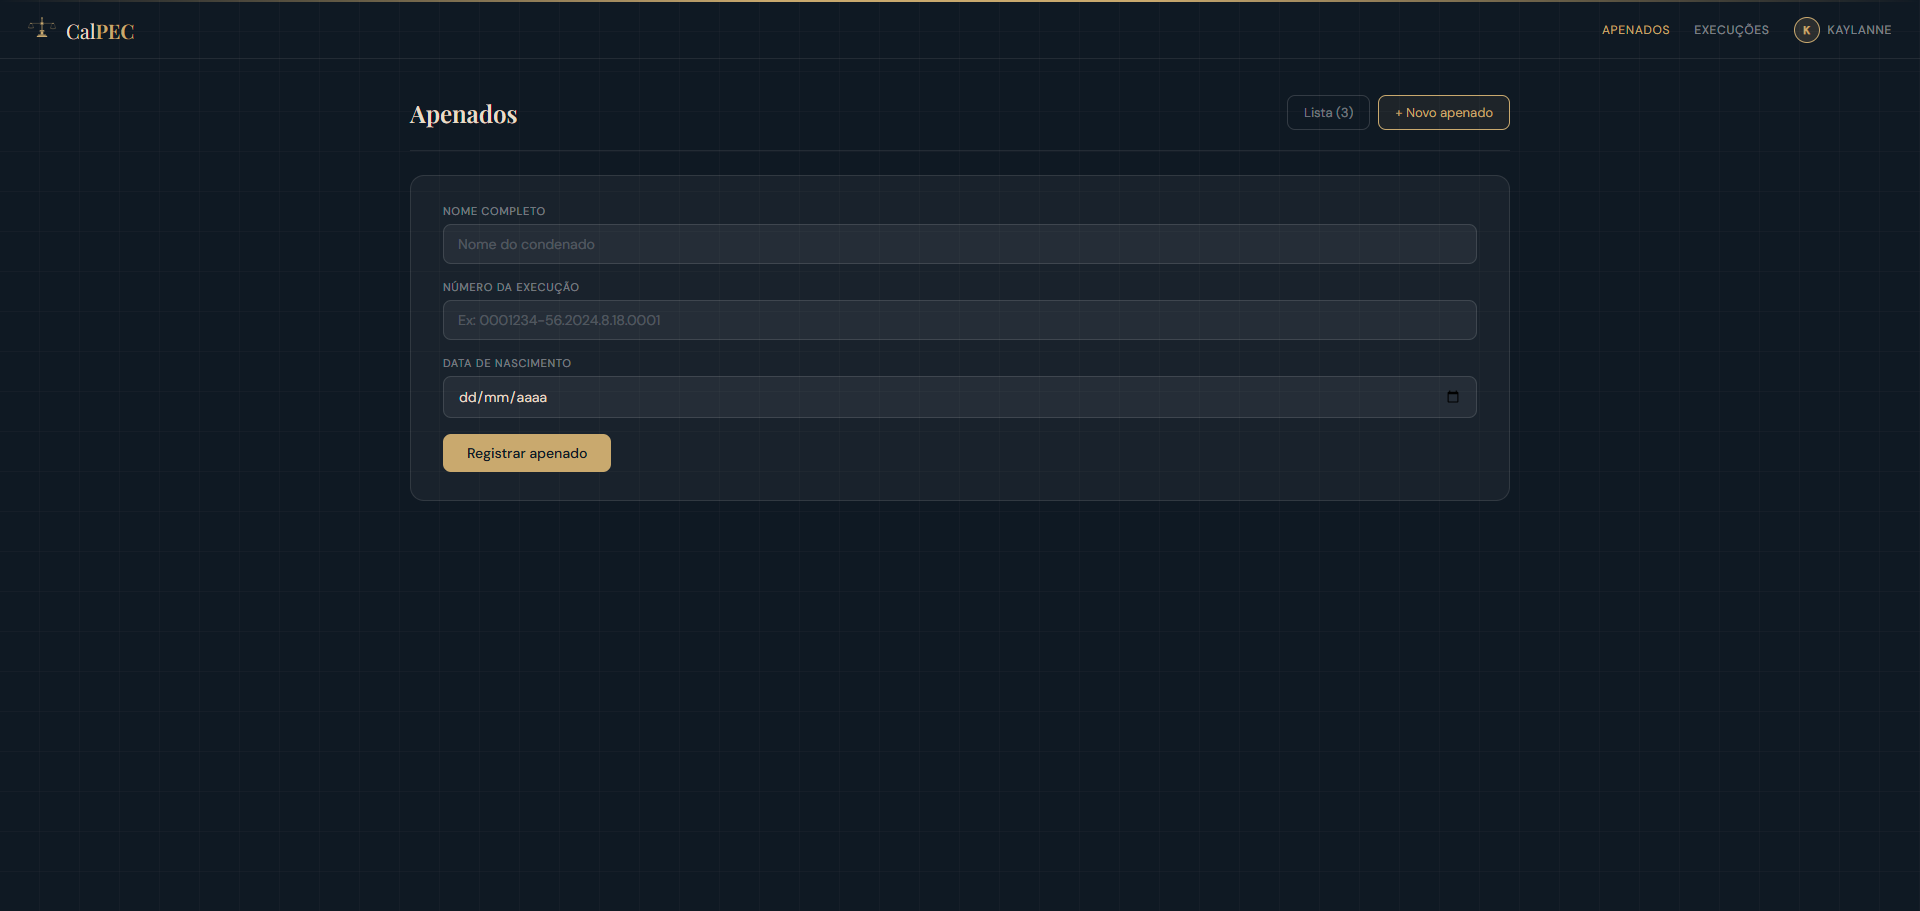
\includegraphics[width=1.0\textwidth]{imagens/prototipo/add-apenado.png}
    \end{center}
    \legend{Fonte: Elaborado pelo Autor}
    \label{fig:tela-apenado}
\end{figure}

\begin{figure}[H]
    \caption{Listar Apenados.}
    \begin{center}
        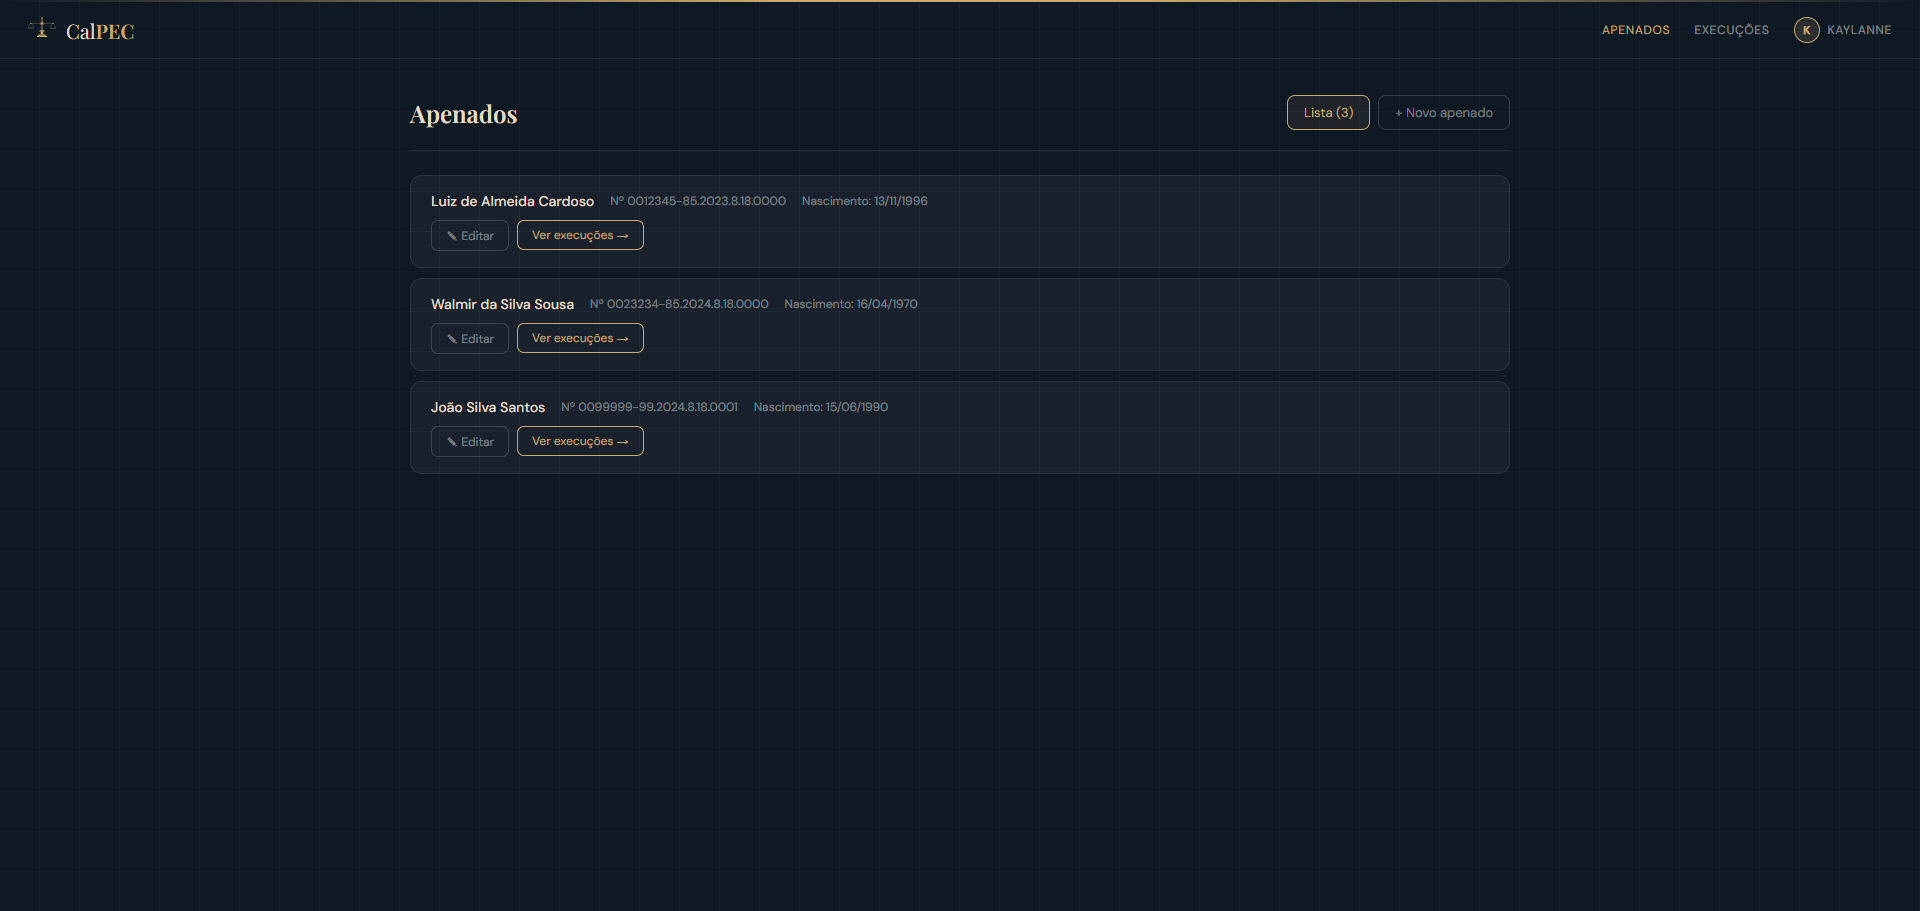
\includegraphics[width=1.0\textwidth]{imagens/prototipo/list-apenados.png}
    \end{center}
    \legend{Fonte: Elaborado pelo Autor}
    \label{fig:tela-listar-apenados}
\end{figure}

\subsection{Editar apenado}
A Figura~\ref{fig:edit-apenado} apresenta a tela de edição dos dados do apenado. Ao clicar em "editar" no apenado desejado, o formulário de edição se expande, permitindo a atualização das informações cadastradas. Essa funcionalidade garante que os dados do apenado possam ser corrigidos ou atualizados sempre que necessário, sem a necessidade de um novo cadastro.

\begin{figure}[H]
    \caption{Editar Apenado.}
    \begin{center}
        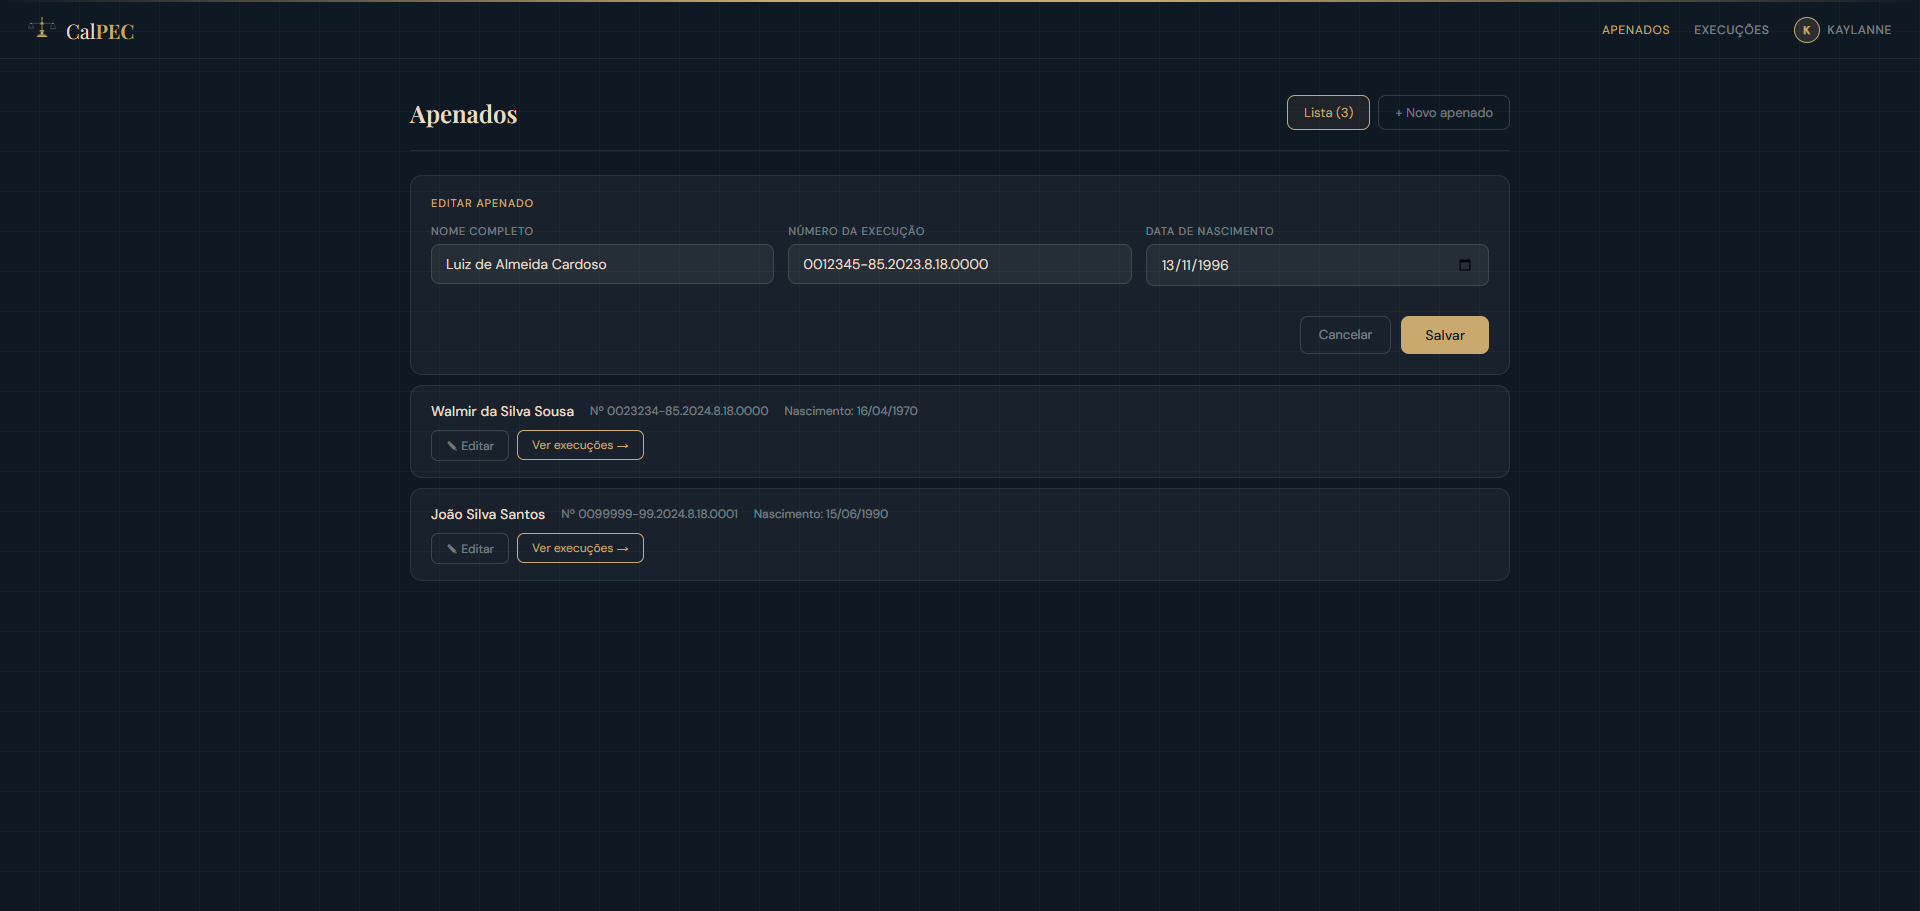
\includegraphics[width=1.0\textwidth]{imagens/prototipo/edit-apenado.png}
    \end{center}
    \legend{Fonte: Elaborado pelo Autor}
    \label{fig:edit-apenado}
\end{figure}

\subsection{Listar execuções}
A Figura~\ref{fig:list-execucoes} exibe a tela de listagem das execuções criminais cadastradas no sistema. O usuário tem acesso a todas as execuções registradas, podendo visualizar o status de progressão de cada uma, acessar o relatório completo ou registrar novas remições, mantendo o acompanhamento contínuo do cumprimento da pena.

\begin{figure}[H]
    \caption{Listar Execuções.}
    \begin{center}
        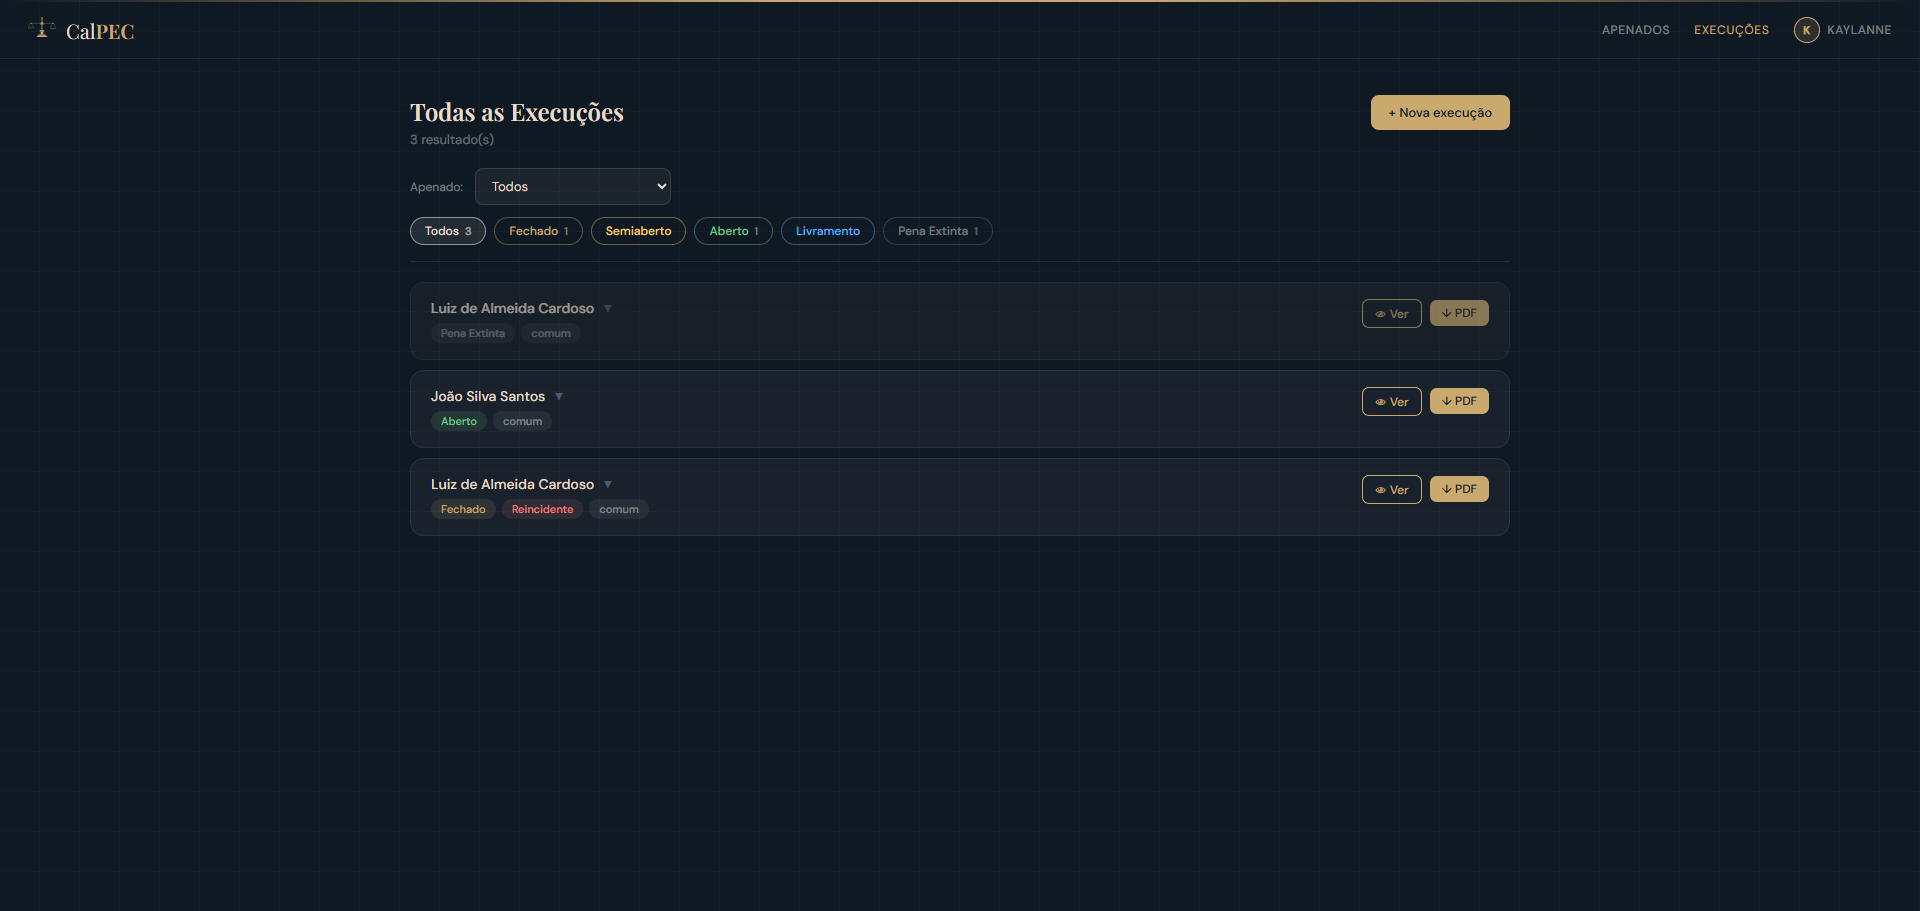
\includegraphics[width=1.0\textwidth]{imagens/prototipo/list-execucoes.png}
    \end{center}
    \legend{Fonte: Elaborado pelo Autor}
    \label{fig:list-execucoes}
\end{figure}

\subsection{Registrar execução criminal}
Ao clicar em "nova execução", o sistema navega até a página de registro penal, conforme a Figura~\ref{fig:tela-execucao}. Na presente página, antes de preencher os campos, o usuário primeiramente realiza a busca pelo apenado que deseja criar a execução. A busca pode ser realizada por meio do nome ou número do processo. No registro de execução, existem todos os campos necessários para gerar o processo de execução penal: tempo total da pena (pena-base definida), natureza do crime, a opção de marcação se o réu é reincidente ou primário, a data de início da pena, a data de início e fim da detração, os campos de remições iniciais, bem como o preenchimento dos campos de benefícios por trabalho, estudo e leitura.

\begin{figure}[H]
    \caption{Registrar Execução Criminal.}
    \begin{center}
        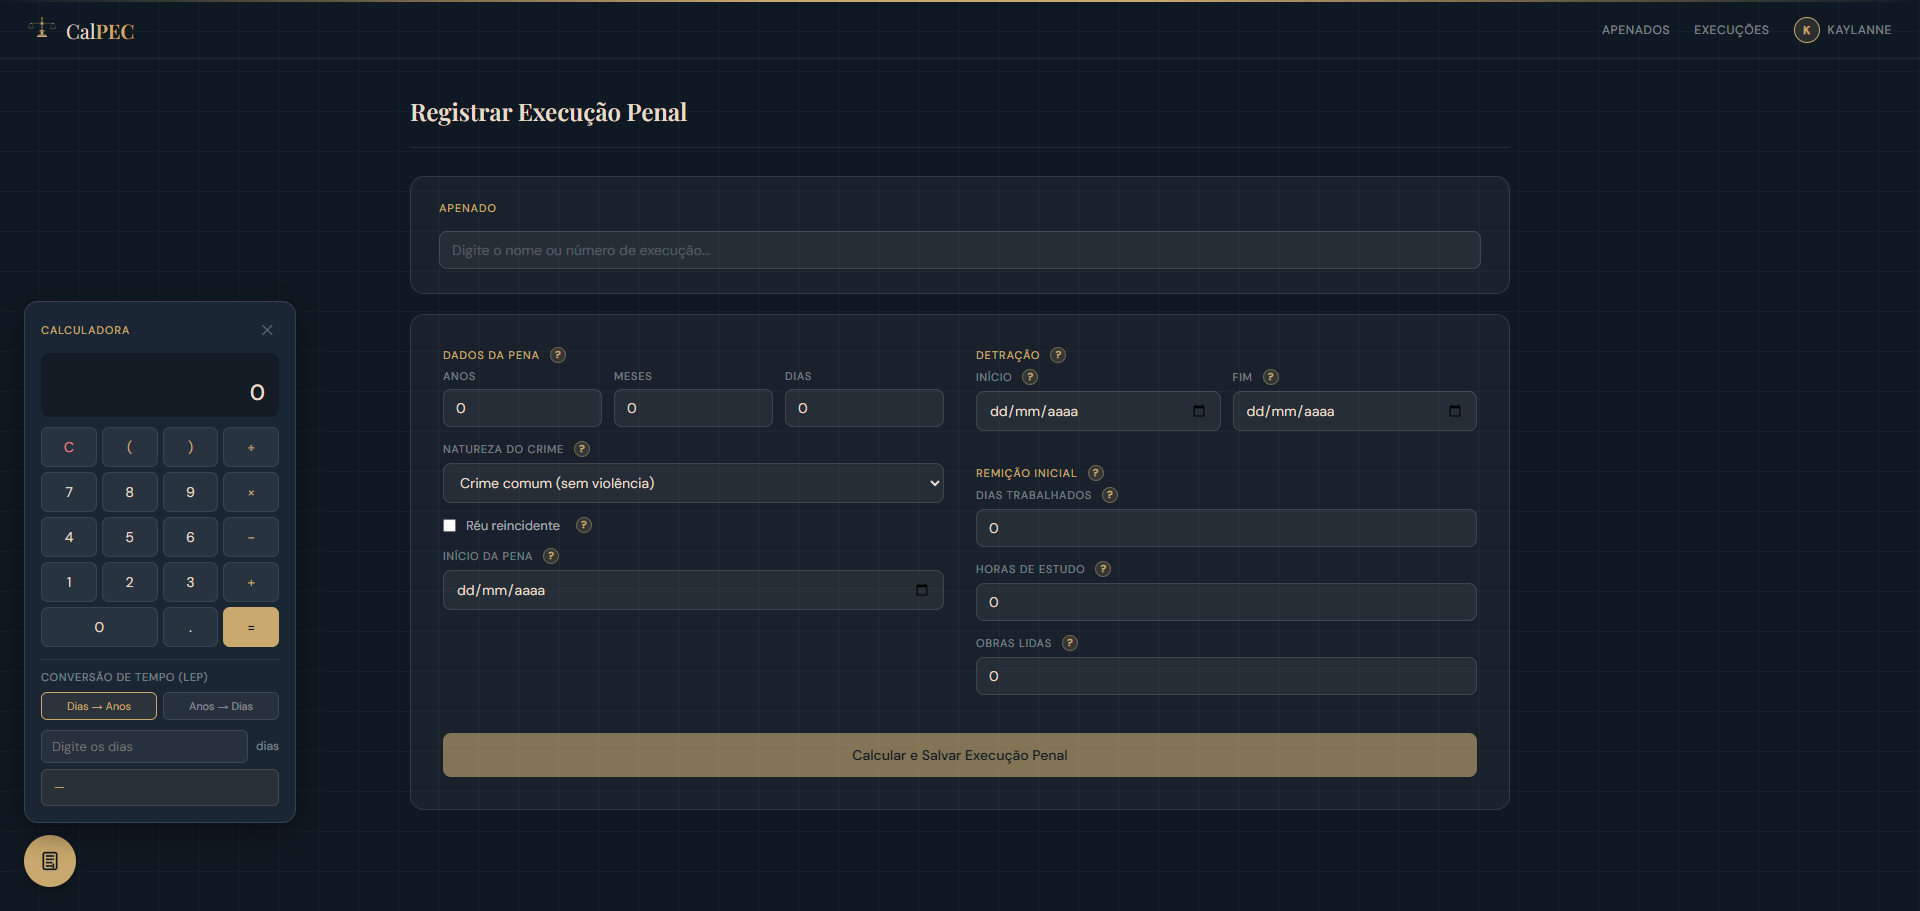
\includegraphics[width=1.0\textwidth]{imagens/prototipo/add-execucao.png}
    \end{center}
    \legend{Fonte: Elaborado pelo Autor}
    \label{fig:tela-execucao}
\end{figure}

Além disso, o sistema tem a opção de usar uma calculadora que realiza cálculos e conversões de dias para anos ou vice-versa, por meio do botão flutuante no canto inferior esquerdo da tela. Ademais, o sistema realiza o cálculo automático da progressão de regime, data de término da pena e status de progressão, com base nas informações preenchidas.

\subsection{Editar execução criminal}
A Figura~\ref{fig:edit-execucao} apresenta a tela de edição de uma execução criminal já cadastrada. Ao clicar em "editar execução", o formulário de edição se expande, permitindo a atualização dos dados registrados. Essa funcionalidade possibilita a correção ou atualização de qualquer informação da execução sem a necessidade de um novo cadastro.

\begin{figure}[H]
    \caption{Editar Execução Criminal.}
    \begin{center}
        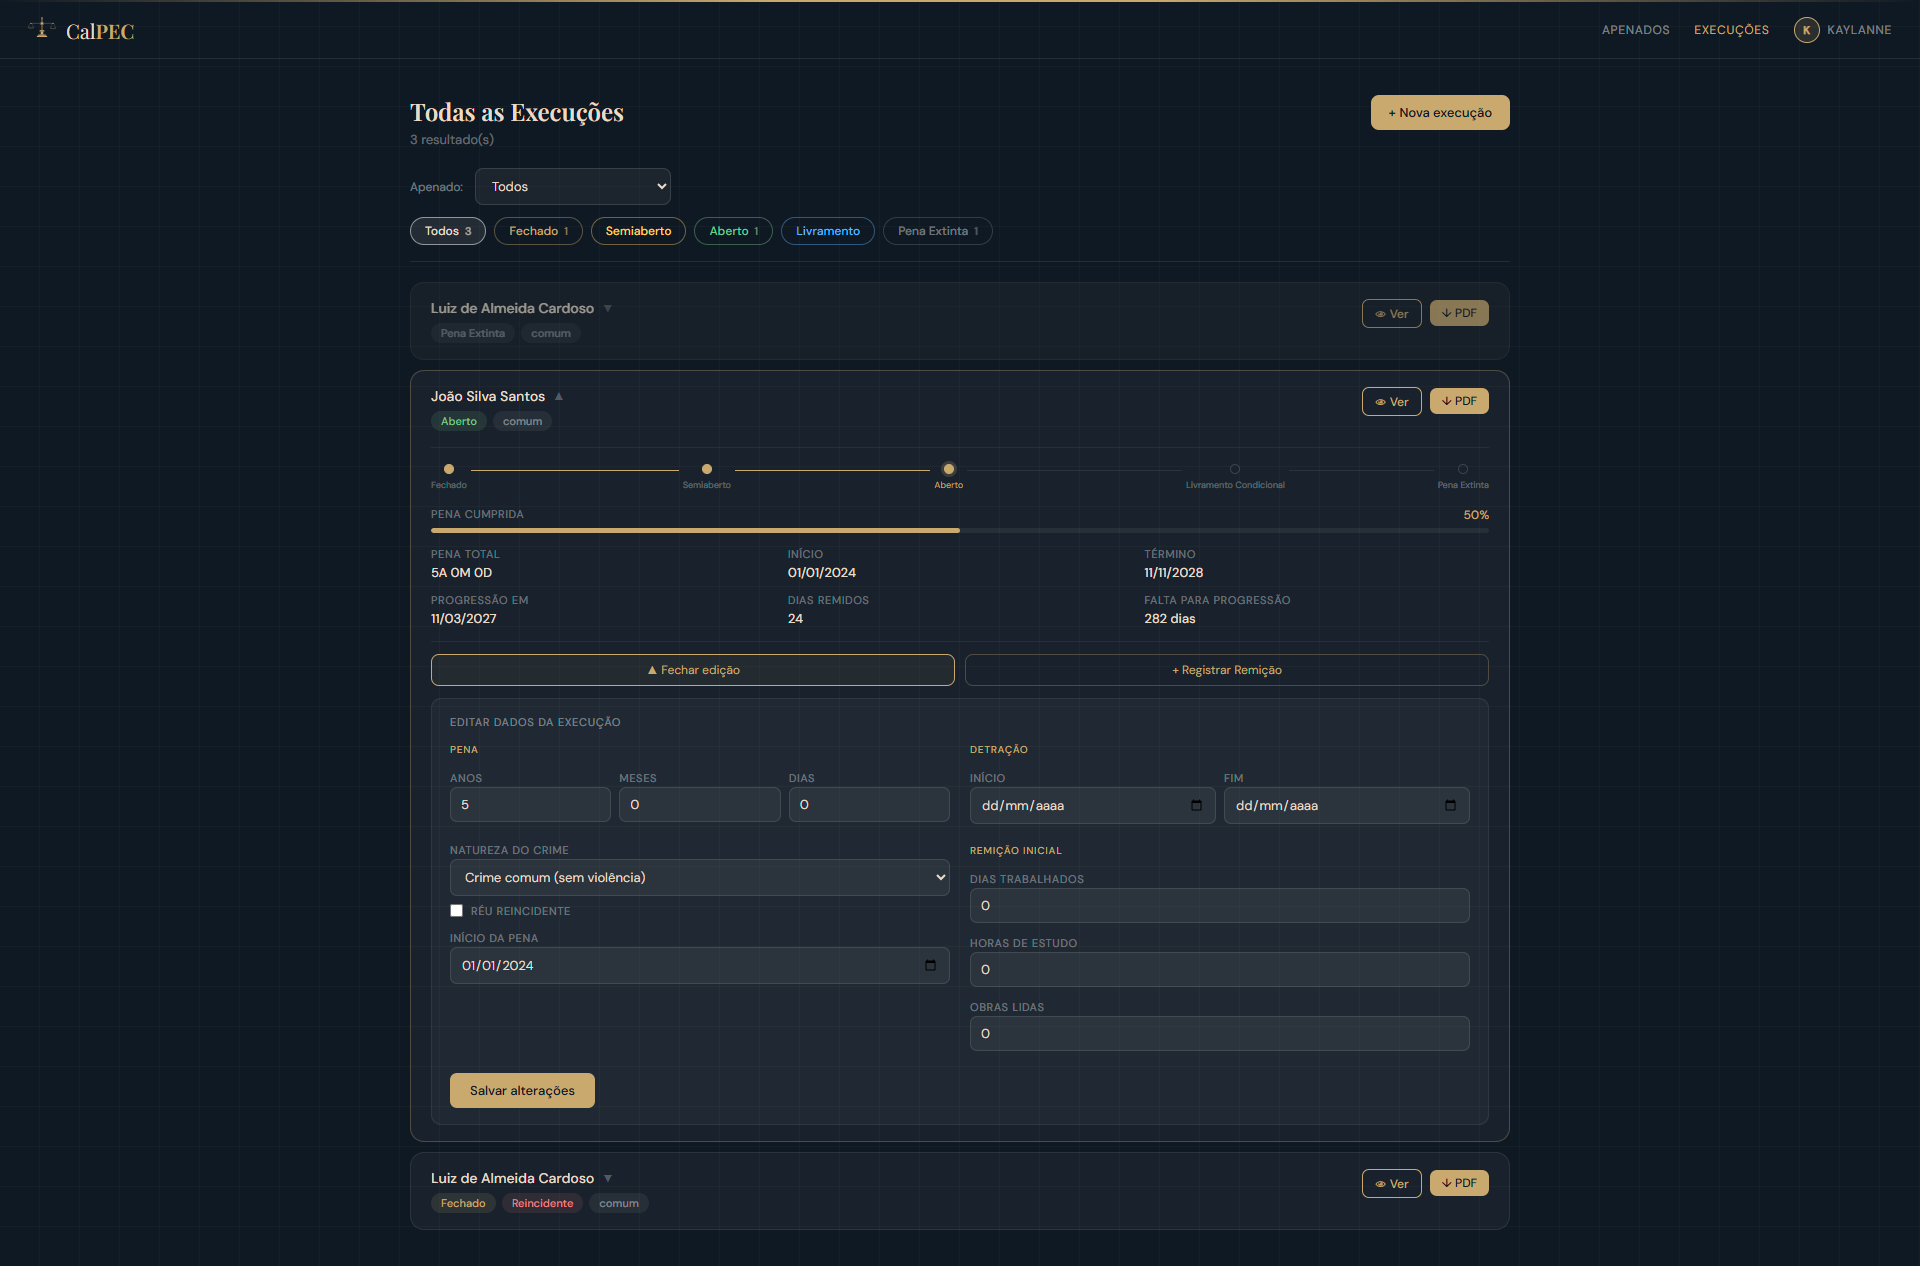
\includegraphics[width=1.0\textwidth]{imagens/prototipo/edit-execucao.png}
    \end{center}
    \legend{Fonte: Elaborado pelo Autor}
    \label{fig:edit-execucao}
\end{figure}

\subsection{Adicionar remição}
A Figura~\ref{fig:add-remicao} exibe a tela de registro de uma nova remição. O advogado informa o tipo de remição (trabalho, estudo ou leitura), a quantidade correspondente e o período de referência. Ao confirmar o registro, o sistema recalcula automaticamente a progressão de regime e o término da pena, atualizando o status da execução com base na nova remição computada.

\begin{figure}[H]
    \caption{Adicionar Remição.}
    \begin{center}
        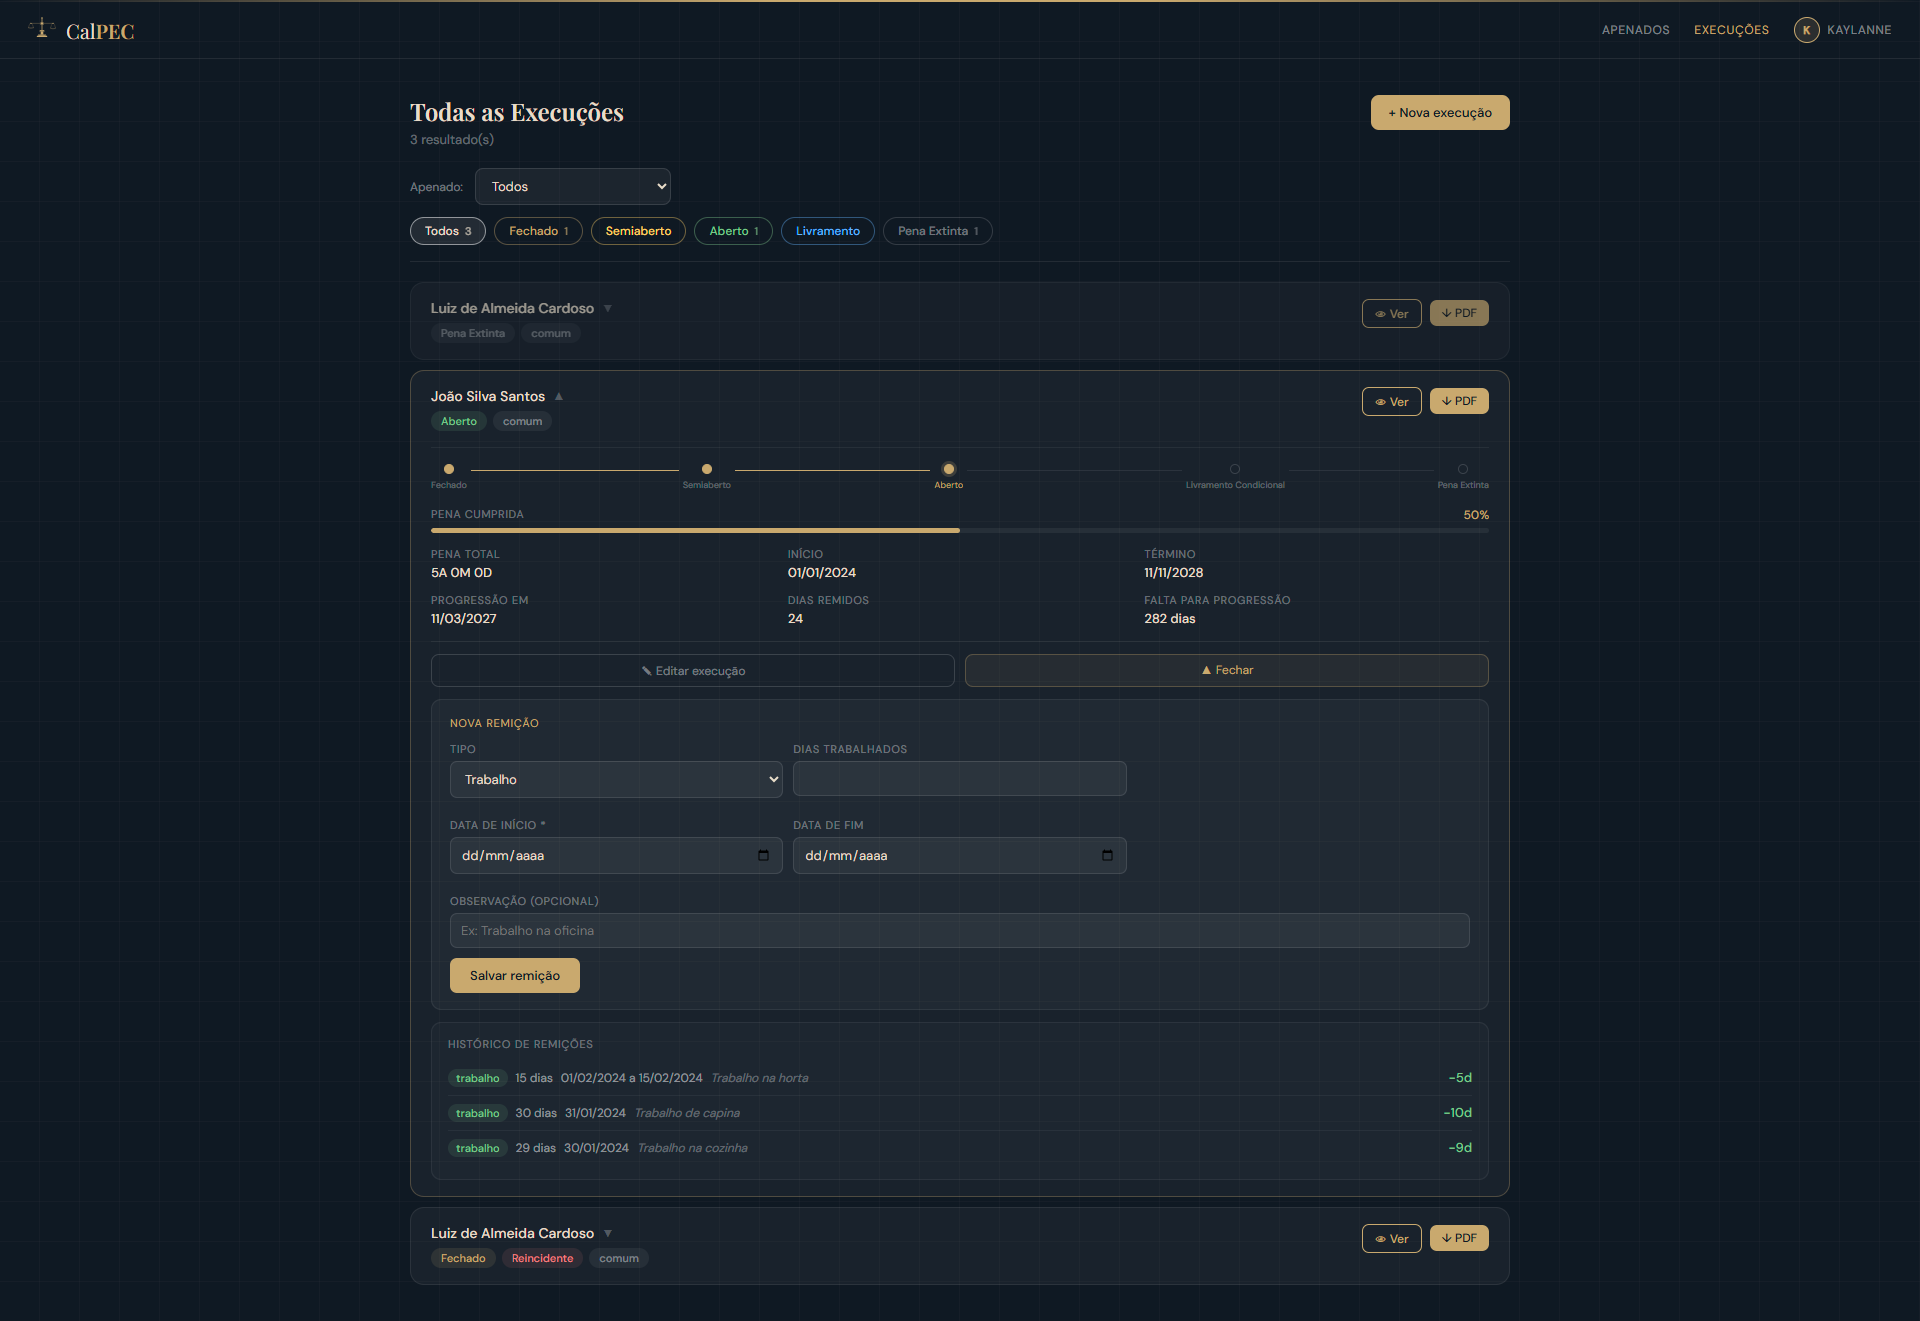
\includegraphics[width=1.0\textwidth]{imagens/prototipo/add-remicao.png}
    \end{center}
    \legend{Fonte: Elaborado pelo Autor}
    \label{fig:add-remicao}
\end{figure}

\subsection{Visualizar relatório}
A Figura~\ref{fig:view-relatorio} apresenta a tela de visualização do relatório da execução. Gerado automaticamente pelo sistema, o relatório reúne em formato de documento formal todas as informações da execução: dados do apenado, pena total, detração, remições computadas, regime atual, data de progressão e data de término da pena.

\begin{figure}[H]
    \caption{Visualizar Relatório.}
    \begin{center}
        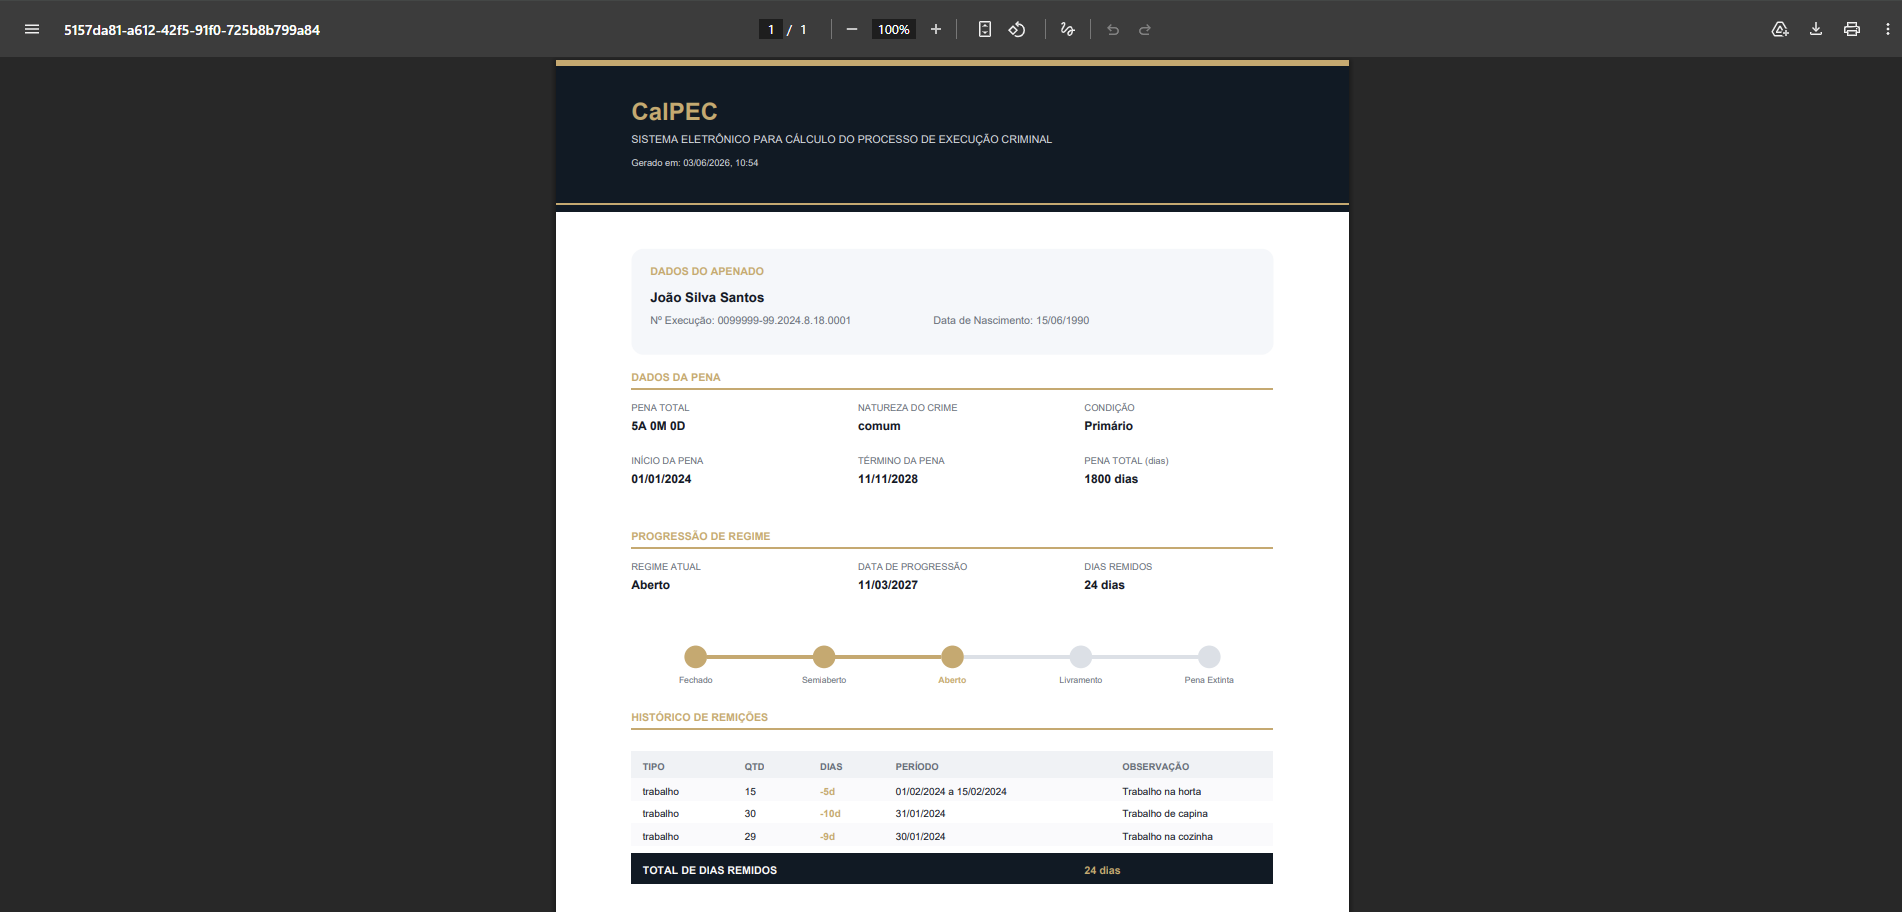
\includegraphics[width=1.0\textwidth]{imagens/prototipo/view-relatorio.png}
    \end{center}
    \legend{Fonte: Elaborado pelo Autor}
    \label{fig:view-relatorio}
\end{figure}

\subsection{Perfil do Usuário}
A Figura~\ref{fig:perfil-user} exibe a tela de perfil do usuário logado, responsável pelo uso do sistema. Nela são apresentados os dados cadastrais do usuário, como nome, e-mail, CPF e número da OAB, permitindo a visualização e eventual atualização das informações de cadastro diretamente pela plataforma. Essa aba permite que o usuário mantenha seus dados atualizados, com campos editáveis caso o usuário necessite de alterações.

\begin{figure}[H]
    \caption{Perfil do Usuário.}
    \begin{center}
        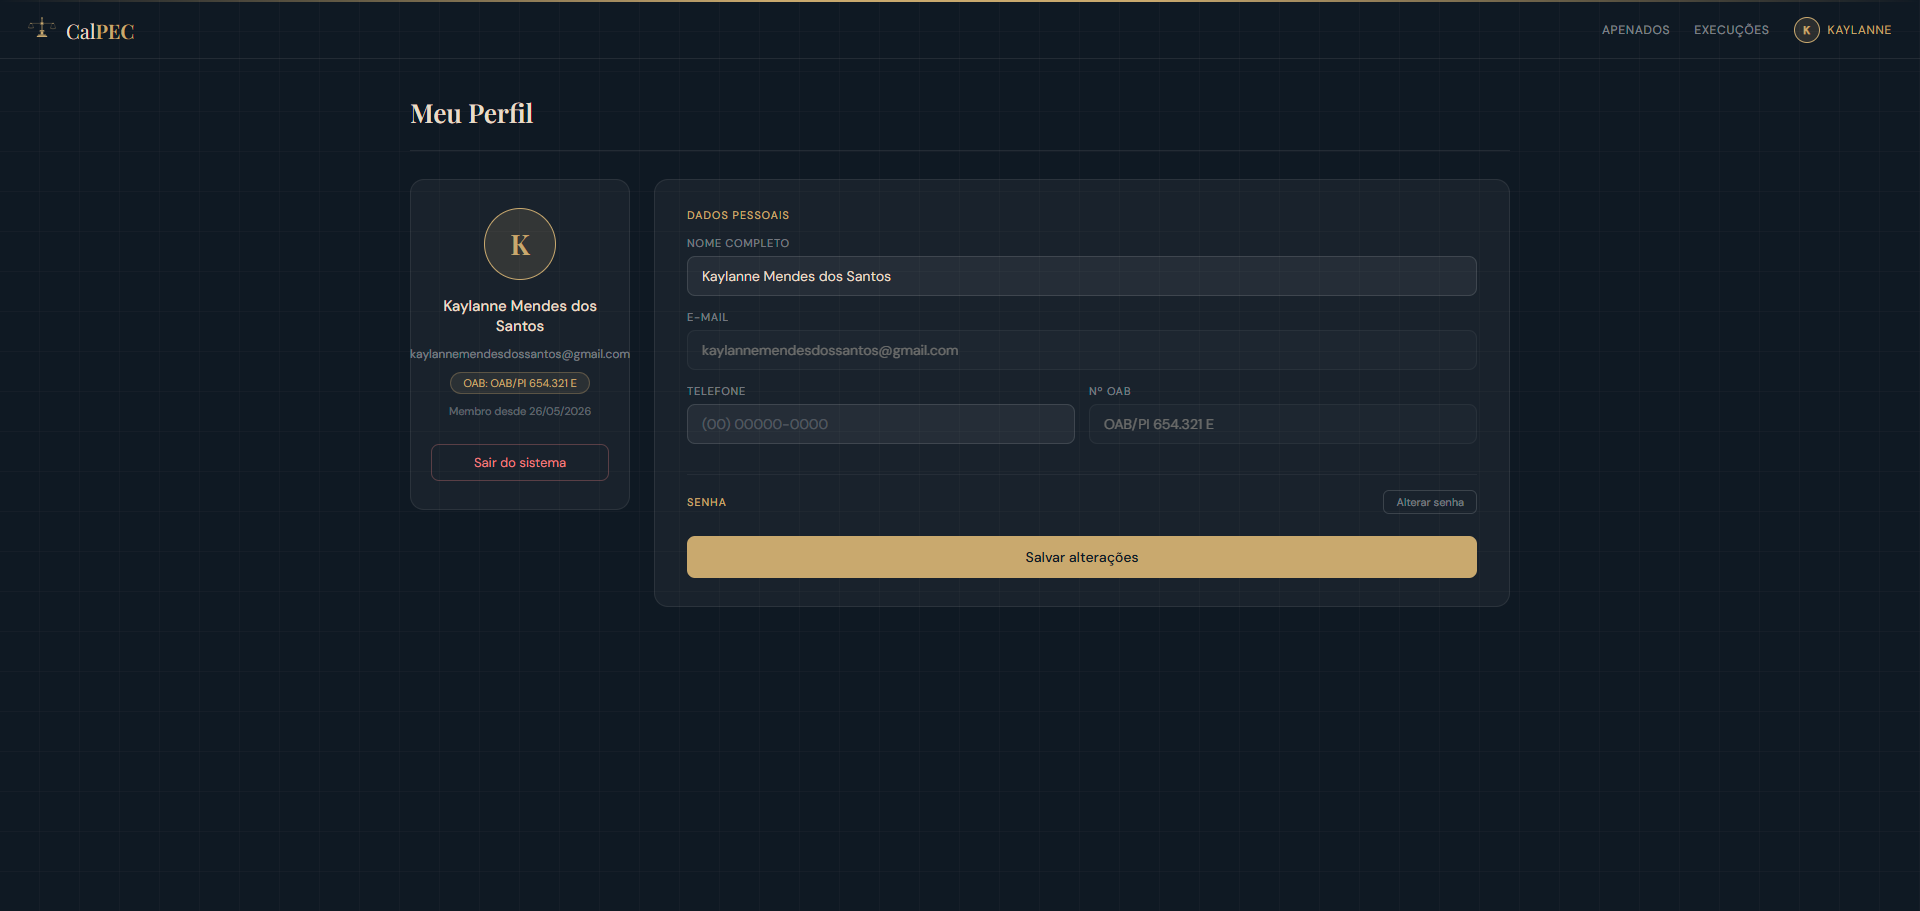
\includegraphics[width=1.0\textwidth]{imagens/prototipo/perfil-user.png}
    \end{center}
    \legend{Fonte: Elaborado pelo Autor}
    \label{fig:perfil-user}
\end{figure}

\section{EXEMPLO PRÁTICO}
Diante do cenário apresentado, faz-se necessário explicar como funciona o fluxo do processo de execução penal do início ao fim. Inicialmente, identificam-se os dados essenciais: nome do condenado, a natureza do crime cometido, o tempo total de pena, regime inicial e data da prisão efetiva. A Vara Criminal expede a guia de execução criminal (GEP), contendo regimes, antecedentes, certidões. Essa guia faz parte da Vara de execuções penais, que autua no Processo de Execução Penal (PEC), por meio do sistema eletrônico SEEU. O exemplo a seguir 
ilustra como esse cálculo é realizado de forma manual, processo que o CalPEC automatiza, eliminando a necessidade de operações manuais e reduzindo a margem de erro.\cite{cnjSEEU}

Por conseguinte, a GEP é enviada ao juízo de execução penal, que realiza a abertura do processo de execução penal (PEC). Com a abertura da PEC, o advogado responsável pelo caso tem acesso aos dados: pena total, data de início, regime, detração, datas-base para benefícios (progressão, livramento condicional, saída temporária). 

Durante o processo de execução, o defensor acompanha a conduta do apenado, requer remição por trabalho ou estudo, monitora progressão de regime, indulto/comutação, e atua em casos como falta grave, unificação de penas ou retificação de cálculo. Por fim, o advogado pode requerer a extinção da pena e expedição do alvará de soltura.

Por exemplo, José foi condenado a 8 anos de prisão por crime comum (não hediondo), réu primário, de acordo com o CP. José foi preso em flagrante, em prisão provisória por 6 meses, antes da sentença definitiva. Antes de iniciar o cumprimento da pena, o primeiro cálculo solicitado é o cálculo de detração, em compensação pelos dias em que José ficou detido provisoriamente. 
Primeiramente, o defensor de José converte os 6 meses de prisão provisória para dias:
\begin{equation*}
(6\,meses \times 30\,dias = 180 dias)
\end{equation*} 
Assim como converte também o tempo de pena:
\begin{equation*}
(8 anos \times 360 dias =  2880 dias)
\end{equation*} 
Com a compensação da detração sob o tempo de pena, o tempo de pena-base é de 2880 dias, logo:
\begin{equation*}
(2880 dias \text{–} 180 dias = 2700 dias)
\end{equation*}
2700 dias correspondem a 7 anos, logo o regime inicial é o semiaberto, segundo a tipificação do crime e pena-base. De acordo com o art. 112 da LEP, a porcentagem necessária de cumprimento de pena é 16\%(0,16). Para saber o lapso temporal necessário para progressão de regime, o advogado de José usa o valor da pena-base e multiplica pela fração ou porcentagem, resultando em 432 dias restantes para então ele progredir de regime: 
\begin{equation*}
(0{,}16 \times 2700 dias = 432 dias)
\end{equation*}
Durante o cumprimento da pena, José passa a ser acompanhado e a sua conduta observada, realizando atividades que contribuam para remição. José trabalhou por 20 dias por mês, segundo a LEP a cada 3 dias trabalhados, é computado 1 dia de remição. Dessa forma, José terá 80 dias de remição:
\begin{equation*}
(20d \times 12m = 240 dias \;\rightarrow\ 240\,dias \div 3\,dias = 80d)
\end{equation*}
Então, ao calcular-se a remição sob a pena-base, ele terá atualmente 2620 dias restantes para cumprimento de pena total:
\begin{equation*}
(2700\,dias - 80\,dias = 2620dias)
\end{equation*}
Sendo necessários ainda 419 dias para progredir de regime:
\begin{equation*}
(0{,}16 \times 2620\,dias = 419{,}2\,dias \approx 419\,dias)
\end{equation*}
Posteriormente, as remições futuras serão computadas sob a pena sempre que necessário, seguidas de atualizações sempre que houver alterações, podendo haver situações de remição ou de regressão, caso o apenado não pratique as condutas corretas.

\section{TECNOLOGIAS UTILIZADAS}

O desenvolvimento da calculadora de execução criminal envolveu a seleção de tecnologias modernas, levando em consideração não apenas o quesito técnico de adequação ao projeto, mas também a familiaridade e experiência com cada ferramenta escolhida, visando garantir um sistema eficiente e robusto.

Primeiramente, para o desenvolvimento do frontend, foi utilizado o React 18.3.1\cite{react}, biblioteca JavaScript amplamente adotada no desenvolvimento de interfaces web, disponível em \url{https://react.dev}. A escolha se deu pela experiência prévia com a tecnologia em projetos anteriores, o que possibilitou maior segurança no desenvolvimento dos componentes e na gestão do estado da aplicação. O projeto frontend foi estruturado com o Vite 5.2.11\cite{vite}, ferramenta de build moderna que proporciona maior desempenho no desenvolvimento, disponível em \url{https://vitejs.dev}. A aplicação frontend está hospedada na plataforma Vercel\cite{vercel} (\url{https://vercel.com}).

Ademais, para o backend, optou-se pelo framework FastAPI 
0.115.0\cite{fastapi}, baseado em Python 3.13.3, disponível em \url{https://fastapi.tiangolo.com}. A linguagem Python se destacou pela praticidade e pela legibilidade do código, facilitando a implementação da lógica de negócio responsável pelos cálculos de execução penal (operações que envolvem datas, frações e percentuais) que exigem precisão e clareza no código. O serviço de backend está hospedado na plataforma Render\cite{render} (\url{https://render.com}).

Por fim, para o banco de dados, definiu-se o PostgreSQL 
17.6\cite{postgresql}, sistema gerenciador de banco de dados relacional robusto e amplamente utilizado em aplicações de produção, disponível em \url{https://www.postgresql.org}. A escolha se deve à vivência anterior com a tecnologia, o que permitiu uma modelagem eficiente, garantindo a integridade e a segurança dos dados armazenados. O banco de dados está hospedado na plataforma Supabase\cite{supabase} 
(\url{https://supabase.com}), que oferece uma camada gerenciada sobre o PostgreSQL, facilitando a administração e o acesso remoto com segurança.

\section{PRIVACIDADE E SEGURANÇA DE DADOS}

Por lidar com dados sensíveis de pessoas condenadas, o CalPEC foi desenvolvido com atenção aos princípios estabelecidos pela Lei Geral de Proteção de Dados (LGPD), Lei nº 13.709/2018 \cite{lgpd}. O sistema adota o princípio da minimização de dados, coletando apenas as informações estritamente necessárias para o funcionamento da aplicação: dados de identificação do advogado (nome, e-mail, CPF, número da OAB e telefone) e dados do apenado (nome, data de nascimento e número de execução). Quanto à segurança das credenciais, as senhas dos usuários são armazenadas em formato de hash, garantindo que, mesmo em caso de acesso indevido ao banco de dados, as senhas originais não possam ser recuperadas.

Como perspectiva de evolução, o sistema prevê a implementação de controle de acesso por perfil de usuário, garantindo que cada advogado visualize exclusivamente os dados que ele mesmo cadastrou, em conformidade com o princípio do acesso restrito previsto na LGPD. Além disso, está prevista a implementação do direito de exclusão de dados pelo titular, bem como a elaboração de uma política de privacidade acessível aos usuários da plataforma.